\documentclass[conference]{IEEEtran}
%\IEEEoverridecommandlockouts
% \usepackage[utf8]{inputenc}
% \usepackage[T1]{fontenc}
% \usepackage[american]{babel}
% \usepackage[center]{caption}
% \usepackage{graphicx}
% \usepackage{listings}
% \usepackage{amsmath,amssymb,exscale}
% \usepackage{blindtext, graphicx}
% \usepackage{verbatim}
% \usepackage{algorithm}
% \usepackage{algpseudocode}
% \usepackage{fancyvrb}
% \usepackage{bera}
% \usepackage{amsmath}
% \usepackage{mathtools}
% \usepackage{lipsum}
% \usepackage[bookmarks=false]{hyperref}
% \usepackage{academicons}
% \usepackage{xcolor}
% \usepackage{tikz}
% \newcommand{\orcid}[1]{\href{https://orcid.org/#1}{\textcolor[HTML]{A6CE39}{\aiOrcid}}}
%\gdef\thesubsection{\thesection.\arabic{subsection}}% rogers
%\gdef\thesectiondis{\Alph{section}}% rogers
%% Load additional packages
%\usepackage{keyval} % Used for passing options to packages
%\usepackage{rotating} % Allows for rotation of images
%\usepackage{lettrine} % Used for lettrines
%\usepackage{verbatim} % Allows for verbatim text and block comments
%\usepackage{pdfpages} % Includes pages of finished PDF files
%\usepackage{setspace} % Allows for control of line spacing
%
% Typeset SI units per ISO standard
\usepackage[mode = math]{siunitx}
\usepackage[T1]{fontenc}
\usepackage[utf8]{inputenc}
\usepackage{mathptmx}
\usepackage{amssymb}
\usepackage{amsmath}
%\usepackage{amsthm}
\usepackage{array}
%\usepackage{biblatex}
%\bibliography{LaTeX/.bib}
%\addbibresource{LaTeX/refs.bib}
\usepackage{cancel}
%\usepackage{caption}
%\usepackage{chagepage}
\usepackage[american]{circuitikz}
%\usepackage{cite}
\usepackage{colortbl}
\usepackage{comment}
%\usepackage{coloremoji}
%\usepackage{empheq}
%\usepackage{enumerate}
%\usepackage{enumitem}
\usepackage{endnotes}
%\usepackage{esint}
\usepackage{etoolbox}
\usepackage{fancyhdr}
%\usepackage{filecontents}
%\usepackage{fontspec}
\usepackage{hanging}
%\usepackage{nomencl}
%\usepackage{fancyref}
\usepackage[bottom=1in, top=1in, right=1in, left=1in]{geometry}                
\usepackage{lastpage}
%\usepackage{listings}
%\usepackage{mathabx}
\usepackage{mathrsfs}
\usepackage{mathtools}
%\usepackage{multicol}
%\usepackage{multido}
\usepackage{pbox}
\usepackage{pdfpages}
\usepackage{pgf}
\usepackage{pgfplots}
%\usepackage{pgf-pie}
\usepackage{pgfplotstable} 
%\usepackage{pgfcalendar}
\usepackage{pdflscape}
%\usepackage{lscape}
%\usepackage{./LaTeX/pgfgantt}
%\usepackage{subfig}
\usepackage{steinmetz}		
\usepackage{textcomp}
\usepackage{tikz}
\usetikzlibrary{decorations.pathmorphing}
\usepackage[absolute,overlay]{textpos}
\usetikzlibrary{calc}
\usetikzlibrary{decorations.markings,positioning,arrows,shapes,patterns}
%\usepackage{./LaTeX/3dplot}
\usetikzlibrary{arrows}
%\usepackage{titling}
\usepackage{varioref}
\usepackage{xcolor}
%\usepackage{../../tools/matlab/mcode}

% page formatting
%\geometry{letterpaper}                   % ... or a4paper or a5paper or ... 
%\geometry{landscape}                % Activate for for rotated page geometry
%\usepackage[parfill]{parskip}    % Activate to begin paragraphs with an empty line rather 		than an indent
\usepackage{graphicx}
%\usepackage{animate}

\usepackage{hyperref}
\hypersetup{
	colorlinks=true, 
	allcolors=magenta
}

%%%%%%%%%%%%%%%%%%%%%%%%%%%%%%%%%%%%%%%%%%%%%%%%%%%%%%%%%%%%%%%%%%%%%%%%%%%%
%%%%%%%%%%%%%%%%%%%%%%%%%%%%%%%%%%%%%%%%%%%%%%%%%%%%%%%%%%%%%%%%%%%%%%%%%%%%
% custom commands
%%%%%%%%%%%%%%%%%%%%%%%%%%%%%%%%%%%%%%%%%%%%%%%%%%%%%%%%%%%%%%%%%%%%%%%%%%%%
%%%%%%%%%%%%%%%%%%%%%%%%%%%%%%%%%%%%%%%%%%%%%%%%%%%%%%%%%%%%%%%%%%%%%%%%%%%%

%%%%%%%%%%%%%%%%%%%%%%%%%%%%%%%%%%%%%%%%%%%%%%%%%%%%%%%%%%%%%%%%%%%%%%%%%%%%
% environments
%%%%%%%%%%%%%%%%%%%%%%%%%%%%%%%%%%%%%%%%%%%%%%%%%%%%%%%%%%%%%%%%%%%%%%%%%%%%
\newcommand{\db}{\text{ dB }}
\newcommand{\dbw}{\text{ dBW }}
\newcommand{\dbsm}{\text{ dBsm }}
\newcommand{\dbm}{\text{ dBm }}
\newcommand{\dbmeter}{\text{ dB (meter) }}
\newcommand{\dbhz}{\text{ dB (Hz)}}
\newcommand{\dbi}{\text{ dBi }}
\newcommand{\mylog}[1]{\ensuremath{\text{log}_{10}\lp#1\rp}}
\newcommand{\equals}{=}
\newcommand{\eq}[1]{\begin{align*}#1\end{align*}} % Quick align environment
\newcommand{\eqn}[1]{\begin{align}#1\end{align}} % Quick align environment
\newcommand{\feq}[1]{\begin{flalign*}#1\end{flalign*}} % Quick align environment
\newcommand{\feqn}[1]{\begin{flalign}#1\end{flalign}} % Quick align environment
\newcommand{\en}[2][1)]{\begin{enumerate}[#1]#2\end{enumerate}} % quick enumerate environment
\newcommand{\itm}[1]{\begin{itemize}#1\end{itemize}} % quick enumerate environment
\newcommand{\tb}[3]{\begin{textblock}{#1}(#2)#3\end{textblock}} % quick enumerate environment
\newcommand{\lp}{\left(}  % resized parentheses
\newcommand{\rp}{\right)}
\newcommand{\lb}{\left[}  % resized brackets
\newcommand{\rb}{\right]}
\newcommand{\lbr}{\left\lbrace}  % resized brackets
\newcommand{\rbr}{\right\rbrace}
\newcommand{\nn}{\nonumber}  %skip numbering on line space in equation array
\newcommand{\suml}[2]{\ensuremath{\sum\limits_{#1}^{#2}}}
\newcommand{\mybox}[2]{\begin{center}\fbox{\begin{minipage}{{#1}\linewidth}\vspace{-4mm}\begin{center}{#2}\end{center}\vspace{-4pt}\end{minipage}}\end{center}} % put a box around just about anything
\newcommand{\boxeqn}[1]{\begin{empheq}[box=\fbox]{align}#1\end{empheq}} % the better box
\newcommand{\boxeq}[1]{\begin{empheq}[box=\fbox]{align*}#1\end{empheq}} % the better box
\newcommand*\wfbox[1]{\fbox{\hspace{10pt#1\hspace{12pt}}}}
\newcommand*\cfbox[1]{\fbox{\hspace{10pt#1\hspace{18pt}}}}
\newcommand\scalemath[2]{\scalebox{#1}{\mbox{\ensuremath{\displaystyle #2}}}} 
\newenvironment{changemargin}[2]{%
  \begin{list}{}{%
    \setlength{\topsep}{0pt}%
    \setlength{\leftmargin}{#1}%
    \setlength{\rightmargin}{#2}%
    \setlength{\listparindent}{\parindent}%
    \setlength{\itemindent}{\parindent}%
    \setlength{\parsep}{\parskip}%
  }%
  \item[]}{\end{list}}
%\newcommand{\sgn}[1]{\ensuremath{\text{sgn}\lp{#1}\rp}}
\newcommand{\hp}[1]{\hphantom{#1}}


%%%%%%%%%%%%%%%%%%%%%%%%%%%%%%%%%%%%%%%%%%%%%%%%%%%%%%%%%%%%%%%%%%%%%%%%%%%%
% math symbol shortcuts
%%%%%%%%%%%%%%%%%%%%%%%%%%%%%%%%%%%%%%%%%%%%%%%%%%%%%%%%%%%%%%%%%%%%%%%%%%%%
\newcommand\gauss[2]{%
	1/(#2*sqrt(2*pi))*exp(-((x-#1)^2)/(2*#2^2))
		}
		
\newcommand{\clight}{\ensuremath{3\ee{8}\text{m/s}}}
\newcommand{\partd}[2]{\dfrac{\partial{#1}}{\partial{#2}}}
\newcommand{\deriv}[2]{\dfrac{\text{d}#1}{\text{d}#2}}
\newcommand{\ee}[1]{\ensuremath{\times 10^{#1}}}
\newcommand{\inv}[1]{{#1}^{\text{\scriptsize{-$1$}}}}
%\newcommand{\degrees}{\ensuremath{^\circ}}
\newcommand{\mydeg}{\ensuremath{^\circ}}
\newcommand{\mycdot}{\lower0.25ex\hbox{\text{\LARGE{${\cdot}$}}}}
\newcommand{\matlab}{\ensuremath{\mbox{MATLAB}^{\mbox{\tiny\textregistered}}\hspace{2pt} }}
%\newcommand{\dydx}{\ensuremath{\frac{dy}{dx}}}
\newcommand{\sr}{\ensuremath{S\left(\vec{r}\right)}}
\newcommand{\curl}{\ensuremath{\nabla \times}}
%\newcommand{\tcurl}{\ensuremath{\nabla_{t} \times}}
\newcommand{\dive}{\ensuremath{\nabla \cdot}}
%\newcommand{\bE}{\mathbf{E}}
%\newcommand{\bH}{\mathbf{H}}
\newcommand{\expj}[1]{\ensuremath{e^{-jk_0{#1}}}}
%\newcommand{\sme}{\ensuremath{\sqrt{\mu_0\epsilon_0}}}
\newcommand{\e}[1]{e^{#1}}
\renewcommand\Re{\operatorname{Re}}
\renewcommand\Im{\operatorname{Im}}
%\newcommand{\tlap}{\ensuremath{\nabla^2_t}}
%\newcommand{\tgm}{\ensuremath{\tau_{gm}}}
%\newcommand{\tge}{\ensuremath{\tau_{ge}}}
%\newcommand{\et}{\ensuremath{\varepsilon_t}}
%\newcommand{\ez}{\ensuremath{\varepsilon_z}}
%\newcommand{\eg}{\ensuremath{\varepsilon_g}}
%\newcommand{\vrho}{\ensuremath{\vec{\rho}}}
\newcommand{\jvec}{\ensuremath{\vec{J}}}
\newcommand{\evec}{\ensuremath{\vec{E}}}
\newcommand{\hvec}{\ensuremath{\vec{H}}}
%\newcommand{\ve}{\varepsilon}
%\newcommand{\etez}{\ensuremath{\frac{\varepsilon_t}{\varepsilon_z}}}
%\newcommand{\ezet}{\ensuremath{\frac{\varepsilon_z}{\varepsilon_t}}}
%\newcommand{\mtmz}{\ensuremath{\frac{\mu_t}{\mu_z}}}
%\newcommand{\mzmt}{\ensuremath{\frac{\mu_z}{\mu_t}}}
\newcommand{\zhat}{\ensuremath{\mathbf{\hat{z}}}}
\newcommand{\yhat}{\ensuremath{\mathbf{\hat{y}}}}
\newcommand{\xhat}{\ensuremath{\mathbf{\hat{x}}}}
%\newcommand{\lamr}{\ensuremath{\lambda_{\rho}}}
%\newcommand{\vlamr}{\ensuremath{\vec{\lambda}_{\rho}}}
%\newcommand{\vlam}{\ensuremath{\vec{\lambda}}}
%\newcommand{\lamy}{\ensuremath{{\lambda}_{y}}}
%\newcommand{\lamx}{\ensuremath{\lambda_{x}}}
%\newcommand{\lamz}{\ensuremath{\lambda_z}}
%\newcommand{\lamzpsi}{\ensuremath{\lambda_{z\psi_{g}}}}
%\newcommand{\lamzth}{\ensuremath{\lambda_{z\theta_{g}}}}
%\newcommand{\lamzpsiu}{\ensuremath{\lambda_{z\psi}}}
%\newcommand{\lamzthu}{\ensuremath{\lambda_{z\theta}}}
%\newcommand{\lamylth}{\ensuremath{\lambda_{y_{l\theta}}}}
%\newcommand{\lamylpsi}{\ensuremath{\lambda_{y_{l\psi}}}}
%\newcommand{\tgetgm}{\ensuremath{\lp \tge + \tgm \rp}}
%\newcommand{\kxm}{\ensuremath{k_{xm}}}
%\newcommand{\kxn}{\ensuremath{k_{xn}}}
%\newcommand{\kym}{\ensuremath{k_{ym}}}
%\newcommand{\kyn}{\ensuremath{k_{yn}}}
%\newcommand{\kya}{\ensuremath{k_{y\alpha}}}

% Resistors/Voltages
\newcommand{\resn}[1]{\ensuremath{\text{R}_{\text{#1}}}}
\newcommand{\myr}[1]{\ensuremath{\text{R}_{\text{#1}}}}
\newcommand{\vn}[1]{\ensuremath{\text{V}_{\text{#1}}}}
\newcommand{\myv}[1]{\ensuremath{\text{V}_{\text{#1}}}}
\newcommand{\myi}[1]{\ensuremath{\text{I}_{\text{#1}}}}
\newcommand{\myp}[1]{\ensuremath{\text{P}_{\text{#1}}}}
\newcommand{\myz}[1]{\ensuremath{\text{Z}_{\text{#1}}}}
\newcommand{\myg}[1]{\ensuremath{\text{G}_{\text{#1}}}}
\newcommand{\myl}[1]{\ensuremath{\text{L}_{\text{#1}}}}
\newcommand{\myc}[1]{\ensuremath{\text{C}_{\text{#1}}}}
\newcommand{\ohms}{\ensuremath{\Omega} }
\newcommand{\mohms}{\ensuremath{\text{m}\Omega} }
\newcommand{\kohms}{\ensuremath{\text{k}\Omega} }
\newcommand{\volts}{\text{V }}
\newcommand{\vrms}{\ensuremath{\text{V}_{\text{RMS }}}}
\newcommand{\kvrms}{\ensuremath{\text{V}_{\text{RMS }}}}
\newcommand{\kvolts}{\text{kV }}
\newcommand{\mvolts}{\text{mV }}
\newcommand{\amps}{\text{A }}
\newcommand{\kamps}{\text{kA }}
\newcommand{\arms}{\ensuremath{\text{A}_{\text{RMS }}}}
\newcommand{\mamps}{\text{mA }}
\newcommand{\watts}{\text{W }}
\newcommand{\mwatts}{\text{mW }}
\newcommand{\kwatts}{\text{kW }}
\newcommand{\speedc}{\ensuremath{3\ee{8}\text{ m/s}}}
%\renewcommand{\k}{\text{k}}
\newcommand{\m}{\text{m}}
\newcommand{\km}{\text{km}}
\newcommand{\rms}{\text{RMS}}
\newcommand{\hz}{\text{Hz}}
\newcommand{\hertz}{\text{Hz}}

% dyads
%\newcommand{\dyad}[1]{\skew2\overline{\skew2\overline{#1}}}
\newcommand{\dyad}[1]{\raisebox{0pt}{\ensuremath{\smash{\stackrel{\hspace*{1pt}\text{\tiny$\leftrightarrow$}}{#1}}}}}
\newcommand{\dmu}{\raisebox{-1pt}{\ensuremath{\dyad{\mu}}}}
%\newcommand{\dmu}{\ensuremath{\dyad{\mu}}}
\newcommand{\idmu}{\inv{\dmu}}
\newcommand{\dep}{\ensuremath{\dyad{\varepsilon}}}
\newcommand{\idep}{\inv{\dep}}
%\newcommand{\we}{\raisebox{0pt}{\ensuremath{\stackrel{\hspace*{-4.5pt}\text{\tiny$\leftrightarrow$}}{\mathsf{w}_e}}}}
%\newcommand{\weth}{\we^{\raisebox{-3pt}{\hspace{-4pt}\tiny$ \theta $}}}
%\newcommand{\wepsi}{\we^{\raisebox{-3pt}{\hspace{-4pt}\tiny$ \psi $}}}
%\newcommand{\iwe}{\we \hspace*{-3pt}\vphantom{w_e}^{\text{\scriptsize{-$1$}}}}
%\newcommand{\wh}{\raisebox{0pt}{\ensuremath{\stackrel{\hspace*{-4.5pt}\text{\tiny$\leftrightarrow$}}{\mathsf{w}_h}}}}
%\newcommand{\iwh}{\wh \hspace*{-3pt}\vphantom{w_h}^{\text{\scriptsize{-$1$}}}}
%%\newcommand{\dlam}{\ensuremath{\raisebox{1pt}{\ensuremath{\dyad{\lambda}}}}}
%\newcommand{\dlam}{\ensuremath{\raisebox{1pt}{\ensuremath{\stackrel{\raisebox{-3pt}[0pt][2pt]{\tiny$\leftrightarrow$}}{\lambda}}}}}
%\newcommand{\id}{\ensuremath{\raisebox{1pt}{\ensuremath{\stackrel{\raisebox{-2.5pt}[0pt][2pt]{\hspace*{1pt}\tiny$\leftrightarrow$}}{I}}}}}
%\newcommand{\kd}{\ensuremath{\raisebox{1pt}{\ensuremath{\stackrel{\raisebox{-3pt}[0pt][2pt]{\tiny$\leftrightarrow$}}{k}}}}}
%\newcommand{\dlampsi}[1]{\dlam_{\psi}^{\raisebox{-3pt}{\hspace{2pt}\scriptsize$ #1 $}}}
%\newcommand{\dlamth}[1]{\dlam_{\theta}^{\raisebox{-3pt}{\hspace{2pt}\scriptsize$ #1 $}}}

%%%%%%%%%%%%%%%%%%%%%%%%%%%%%%%%%%%%%%%%%%%%%%%%%%%%%%%%%%%%%%%%%%%%%%%%%%%%%
%% spatial domain functions
%%%%%%%%%%%%%%%%%%%%%%%%%%%%%%%%%%%%%%%%%%%%%%%%%%%%%%%%%%%%%%%%%%%%%%%%%%%%%
%\newcommand{\gfpe}{\ensuremath{\vec{G}_{\psi_{e}}}}
%\newcommand{\gfthe}{\ensuremath{\vec{G}_{\theta_{e}}}}
%\newcommand{\gfpsim}{\ensuremath{\vec{G}_{\psi_{h}}}}
%\newcommand{\gfthm}{\ensuremath{\vec{G}_{\theta_h}}}
%\newcommand{\aoone}{A_{o_{1}}}
%\newcommand{\aotwo}{A_{o_{2}}}
%\newcommand{\aoonep}{A_{o_{1}}^{\scalemath{0.60}{+}}}
%\newcommand{\aoonem}{A_{o_{1}}^{\scalemath{0.60}{-}}}
%\newcommand{\aotwop}{A_{o_{2}}^{\scalemath{0.60}{+}}}
%\newcommand{\aotwom}{A_{o_{2}}^{\scalemath{0.60}{-}}}
%\newcommand{\vpsip}{V_{\psi}^{\scalemath{0.60}{+}}}
%\newcommand{\vpsim}{V_{\psi}^{\scalemath{0.60}{-}}}
%\newcommand{\vthp}{V_{\theta}^{\scalemath{0.60}{+}}}
%\newcommand{\vthm}{V_{\theta}^{\scalemath{0.60}{-}}}
%\newcommand{\vpsiep}{V_{\psi_{e}}^{\scalemath{0.60}{+}}}
%\newcommand{\vpsimp}{V_{\psi_{h}}^{\scalemath{0.60}{+}}}
%\newcommand{\vthep}{V_{\theta_{e}}^{\scalemath{0.60}{+}}}
%\newcommand{\vthmp}{V_{\theta_{h}}^{\scalemath{0.60}{+}}}
%\newcommand{\vpsiem}{V_{\psi_{e}}^{\scalemath{0.60}{-}}}
%\newcommand{\vpsimm}{V_{\psi_{h}}^{\scalemath{0.60}{-}}}
%\newcommand{\vthem}{V_{\theta_{e}}^{\scalemath{0.60}{-}}}
%\newcommand{\vthmm}{V_{\theta_{h}}^{\scalemath{0.60}{-}}}
%
%\newcommand{\vpsiemp}{V_{\psi_{(e,h)}}^{\scalemath{0.60}{+}}}
%\newcommand{\vpsiemm}{V_{\psi_{(e,h)}}^{\scalemath{0.60}{-}}}
%\newcommand{\vthemp}{V_{\theta_{(e,h)}}^{\scalemath{0.60}{+}}}
%\newcommand{\vthemm}{V_{\theta_{(e,h)}}^{\scalemath{0.60}{-}}}
%
%
%
%\newcommand{\rpsi}{R_{\psi}}
%\newcommand{\rth}{R_{\theta}}
%\newcommand{\rpsibar}{\overline{R}_{\psi}}
%\newcommand{\rthbar}{\overline{R}_{\theta}}
%
%% exponentials
%\newcommand{\ej}[1]{e^{j{#1}}}
%\newcommand{\ejp}[1]{e^{j{#1}}}
%\newcommand{\ejm}[1]{e^{-j{#1}}}
%\newcommand{\ejplzoned}{\ejp{\lamzpone d}}
%\newcommand{\ejmlzoned}{\ejm{\lamzpone d}}
%\newcommand{\ejplztwod}{\ejp{\lamzptwo d}}
%\newcommand{\ejmlztwod}{\ejm{\lamzptwo d}}
%\newcommand{\dpsi}{D_{\psi}}
%
%% isotropic potentials
%\newcommand{\fa}{F_{\alpha}}
%\newcommand{\lamzz}{\lambda_{z0}}
%\newcommand{\ftfa}{\widetilde{F}_{\alpha}}
%\newcommand{\ftfx}{\widetilde{F}_{x}}
%\newcommand{\ftfy}{\widetilde{F}_{y}}
%\newcommand{\ftfz}{\widetilde{F}_{z}}
%\newcommand{\dftfa}{\widetilde{\widetilde{F}}_{\alpha}}
%\newcommand{\ftw}{\widetilde{w}_{\alpha}}
%\newcommand{\ra}{R_{\alpha}}
%\newcommand{\rabar}{\overline{R}_{\alpha}}
%\newcommand{\va}{v_{\alpha}}

%%%%%%%%%%%%%%%%%%%%%%%%%%%%%%%%%%%%%%%%%%%%%%%%%%%%%%%%%%%%%%%%%%%%%%%%%%%%%
%% fourier transform functions
%%%%%%%%%%%%%%%%%%%%%%%%%%%%%%%%%%%%%%%%%%%%%%%%%%%%%%%%%%%%%%%%%%%%%%%%%%%%%
%
%% theta
%\newcommand{\fttheta}{\ensuremath{\widetilde{\theta}}}
%
%% psi
%\newcommand{\ftpsi}{\ensuremath{\widetilde{\psi}}}
%
%% J
%\newcommand{\ftvj}{\ensuremath{\vec{\widetilde{J}}}}
%\newcommand{\dftj}{\ensuremath{\widetilde{\widetilde{J}}}}
%\newcommand{\ftj}{\ensuremath{\widetilde{J}}}
%\newcommand{\ftjv}{\ensuremath{\vec{\widetilde{J}}}}
%\newcommand{\ftjvec}{\ensuremath{\vec{\widetilde{J}}}}
%
%% GF's - PB
%% % custom 
%%\newcommand{\ftgf}{\stackrel{\raisebox{0.5pt}[0pt][0pt]{$ \vec{}$}} {\stackrel{\raisebox{5.5pt}[0pt][0pt]{\scriptsize$ \hspace*{2pt}\sim $}}{\smash{G}}}}
%% % system
%\newcommand{\ftgfv}{\vec{\skew2\widetilde{G}}}
%\newcommand{\ftgf}{\widetilde{G}}
%\newcommand{\ftgfpsie}{\ftgfv_{\psi_{e}}}
%\newcommand{\ftgfpsiet}{\ftgfv_{\psi_{et}}}
%\newcommand{\ftgfpsiez}{\ftgfv_{\psi_{ez}}}
%\newcommand{\ftgfthe}{\ftgfv_{\theta_{e}}}
%\newcommand{\ftgfthet}{\ftgfv_{\theta_{et}}}
%\newcommand{\ftgfthez}{\ftgfv_{\theta_{ez}}}
%\newcommand{\ftgfpie}{\ftgfv_{\Pi_{e}}}
%\newcommand{\ftgfpiet}{\ftgfv_{\Pi_{et}}}
%\newcommand{\ftgfpiez}{\ftgfv_{\Pi_{ez}}}
%\newcommand{\ftgfphie}{\ftgfv_{\Phi_{e}}}
%\newcommand{\ftgfphiet}{\ftgfv_{\Phi_{et}}}
%\newcommand{\ftgfphiez}{\ftgfv_{\Phi_{ez}}}
%
%\newcommand{\ftgfpsim}{\ftgfv_{\psi_{h}}}
%\newcommand{\ftgfpsimt}{\ftgfv_{\psi_{ht}}}
%\newcommand{\ftgfpsimz}{\ftgfv_{\psi_{hz}}}
%\newcommand{\ftgfthm}{\ftgfv_{\theta_{h}}}
%\newcommand{\ftgfthmt}{\ftgfv_{\theta_{ht}}}
%\newcommand{\ftgfthmz}{\ftgfv_{\theta_{hz}}}
%\newcommand{\ftgfpim}{\ftgfv_{\Pi_{h}}}
%\newcommand{\ftgfpimt}{\ftgfv_{\Pi_{ht}}}
%\newcommand{\ftgfpimz}{\ftgfv_{\Pi_{hz}}}
%\newcommand{\ftgfphim}{\ftgfv_{\Phi_{h}}}
%\newcommand{\ftgfphimt}{\ftgfv_{\Phi_{ht}}}
%\newcommand{\ftgfphimz}{\ftgfv_{\Phi_{hz}}}
%
%%GF dyad
%% % custom ones
%%\newcommand{\ftgfd}{\vphantom{\vec{\stackrel{\sim}{G}}}\stackrel{\raisebox{5.75pt}[0pt][0pt]{\hspace*{2.5pt}\tiny$ \leftrightarrow$}}{\stackrel{\raisebox{5.5pt}[0pt][0pt]{\scriptsize$ \hspace*{2pt}\sim $}}{\smash{G}}}}
%%\newcommand{\ftgfp}{\stackrel{\raisebox{0.5pt}[0pt][0pt]{$ \vec{} $}}{\stackrel{\raisebox{5.5pt}[0pt][0pt]{\scriptsize$ \hspace*{2pt}\sim $}}{\smash{G}}}^{\raisebox{-6pt}{\hspace{0pt}\tiny$ p $}}}
%
%% system ones
%\newcommand{\ftgfd}{\stackrel{\raisebox{-2pt}{\tiny$\hspace*{3pt}\leftrightarrow $}}{\widetilde{G}}}
%\newcommand{\ftgfdp}{\stackrel{\raisebox{-2pt}{\tiny$\hspace*{3pt}\leftrightarrow $}}{\widetilde{G}}^{\raisebox{-4pt}{\scriptsize$ p $}}}
%\newcommand{\ftgfp}{\ftgf^{\raisebox{2pt}{\scriptsize$ p $}}}
%
%
%
%%GF theta-theta and psi-psi vectors for FB
%\newcommand{\ftgfthth}{\ftgf^{\raisebox{2pt}{\tiny$ \theta,\theta $}}}
%\newcommand{\ftgfth}{\ftgfd^{\raisebox{-6pt}{\tiny$ \theta $}}}
%\newcommand{\ftgfpsipsi}{\ftgf^{\raisebox{-1pt}{\tiny$ \psi,\psi $}}}
%\newcommand{\ftgfpsi}{\ftgfd^{\raisebox{-5pt}{\tiny$ \psi$}}}
%\newcommand{\ftgfteztez}{\ftgf^{\raisebox{1pt}{\tiny TE,TE}}}
%\newcommand{\ftgftez}{\ftgf^{\raisebox{1pt}{\tiny TE}}}
%\newcommand{\ftgfdtez}{\ftgfd^{\raisebox{-8pt}{\tiny TE}}}
%\newcommand{\ftgftmztmz}{\ftgf^{\raisebox{1pt}{\tiny TM,TM}}}
%\newcommand{\ftgftmz}{\ftgf^{\raisebox{1pt}{\tiny TM}}}
%\newcommand{\ftgfdtmz}{\ftgfd^{\raisebox{-8pt}{\tiny TM}}}
%
%% little gf's - PB
%\newcommand{\ftlgfpsie}{\ensuremath{\vec{\skew2\widetilde{g}}_{\psi_{e}}}}
%\newcommand{\ftlgfpsiet}{\ensuremath{\vec{\skew2\widetilde{g}}_{\psi_{et}}}}
%\newcommand{\ftlgfpsiez}{\ensuremath{\vec{\skew2\widetilde{g}}_{\psi_{ez}}}}
%\newcommand{\ftlgfpsim}{\ensuremath{\vec{\skew2\widetilde{g}}_{\psi_{h}}}}
%\newcommand{\ftlgfpsimt}{\ensuremath{\vec{\skew2\widetilde{g}}_{\psi_{ht}}}}
%\newcommand{\ftlgfpsimz}{\ensuremath{\vec{\skew2\widetilde{g}}_{\psi_{hz}}}}
%\newcommand{\ftlgfthe}{\ensuremath{\vec{\skew2\widetilde{g}}_{\theta_{e}}}}
%\newcommand{\ftlgfthet}{\ensuremath{\vec{\skew2\widetilde{g}}_{\theta_{et}}}}
%\newcommand{\ftlgfthez}{\ensuremath{\vec{\skew2\widetilde{g}}_{\theta_{ez}}}}
%\newcommand{\ftlgfthm}{\ensuremath{\vec{\skew2\widetilde{g}}_{\theta_{h}}}}
%\newcommand{\ftlgfthmt}{\ensuremath{\vec{\skew2\widetilde{g}}_{\theta_{ht}}}}
%\newcommand{\ftlgfthmz}{\ensuremath{\vec{\skew2\widetilde{g}}_{\theta_{hz}}}}
%\newcommand{\ftlgfpsiem}{\ensuremath{\vec{\skew2\widetilde{g}}_{\psi_{\text{\tiny{(e,h)}}}}}}
%\newcommand{\ftlgfthem}{\ensuremath{\vec{\skew2\widetilde{g}}_{\theta_{\text{\tiny{(e,h)}}}}}}
%
%
%% gf's - generalized
%% % custom ones
%%\newcommand{\ftlgfd}{\stackrel{\stackrel{\raisebox{-1.5pt}{\tiny$ \hspace*{2pt}\leftrightarrow $}}{\raisebox{2.5pt}{\scriptsize$ \hspace*{1pt}\sim $}}}{\smash{g}}}
%%\newcommand{\ftlgfptheed}{\stackrel{\stackrel{\raisebox{-1.5pt}{\tiny$ \hspace*{2pt}\leftrightarrow $}}{\raisebox{2.5pt}{\scriptsize$ \hspace*{1pt}\sim $}}}{\smash{g}}_{\hspace*{-2pt}\tiny\text{$ ee $}}^{\raisebox{-4pt}{\tiny$ p\theta $}}}
%%\newcommand{\ftlgfpthehd}{\stackrel{\stackrel{\raisebox{-1.5pt}{\tiny$ \hspace*{2pt}\leftrightarrow $}}{\raisebox{2.5pt}{\scriptsize$ \hspace*{1pt}\sim $}}}{\smash{g}}_{\hspace*{-2pt}\tiny\text{$ eh $}}^{\raisebox{-4pt}{\tiny$ p\theta $}}}
%%\newcommand{\ftlgfppsieed}{\stackrel{\stackrel{\raisebox{-1.5pt}{\tiny$ \hspace*{2pt}\leftrightarrow $}}{\raisebox{2.5pt}{\scriptsize$ \hspace*{1pt}\sim $}}}{\smash{g}}_{\hspace*{-2pt}\tiny\text{$ ee $}}^{\raisebox{-4pt}{\tiny$ p\psi $}}}
%%\newcommand{\ftlgfppsiehd}{\stackrel{\stackrel{\raisebox{-1.5pt}{\tiny$ \hspace*{2pt}\leftrightarrow $}}{\raisebox{2.5pt}{\scriptsize$ \hspace*{1pt}\sim $}}}{\smash{g}}_{\hspace*{-2pt}\tiny\text{$ eh $}}^{\raisebox{-4pt}{\tiny$ p\psi $}}}
%
%
%%% system ones
%\newcommand{\ftlgfd}{\stackrel{\raisebox{-1.5pt}{\tiny$ \hspace*{2pt}\leftrightarrow $}}{\widetilde{g}}}
%\newcommand{\ftlgfptheed}{\ftlgfd^{\raisebox{-4pt}{\tiny$ p\theta $}}_{\hspace*{-2pt} ee}}
%\newcommand{\ftlgfpthehd}{\ftlgfd^{\raisebox{-4pt}{\tiny$ p\theta $}}_{\hspace*{-2pt} eh}}
%\newcommand{\ftlgfppsieed}{\ftlgfd^{\raisebox{-4pt}{\tiny$ p\psi $}}_{\hspace*{-2pt} ee}}
%\newcommand{\ftlgfppsiehd}{\ftlgfd^{\raisebox{-4pt}{\tiny$ p\psi $}}_{\hspace*{-2pt} eh}}
%
%% general grand daddy
%% % custom
%%\newcommand{\ftlgfpgend}{\stackrel{\stackrel{\raisebox{-1.5pt}{\tiny$ \hspace*{2pt}\leftrightarrow $}}{\raisebox{2.5pt}{\scriptsize$ \hspace*{1pt}\sim $}}}{\smash{g}}_{\hspace*{-2pt}\tiny\text{$ ee,eh $}}^{\raisebox{-4pt}{\tiny$ p\theta,p\psi $}}}
%
%% % system
%\newcommand{\ftlgfpgend}{\ftlgfd^{\raisebox{-4pt}{\tiny$ p\theta,p\psi $}}_{\hspace*{-2pt} ee,eh}}
%
%% other ft relations
%\newcommand{\ftlone}{\ensuremath{\widetilde{L}_1}}
%\newcommand{\ftltwo}{\ensuremath{\widetilde{L}_2}}
%\newcommand{\ftlthree}{\ensuremath{\widetilde{L}_3}}
%\newcommand{\ftlfour}{\ensuremath{\widetilde{L}_4}}
%\newcommand{\ftsone}{\ensuremath{\widetilde{s}_1}}
%\newcommand{\ftstwo}{\ensuremath{\widetilde{s}_2}}
%\newcommand{\ftue}{\ensuremath{\widetilde{u}_e}}
%\newcommand{\ftum}{\ensuremath{\widetilde{u}_h}}
%\newcommand{\ftve}{\ensuremath{\widetilde{v}_e}}
%\newcommand{\ftvm}{\ensuremath{\widetilde{v}_h}}
%\newcommand{\ftphi}{\ensuremath{\widetilde{\Phi}}}
%\newcommand{\ftpi}{\ensuremath{\widetilde{\Pi}}}
%\newcommand{\ftpsioonem}{\ftpsi_{o_{1}}^{\scalemath{0.60}{-}}}
%\newcommand{\ftpsioonep}{\ftpsi_{o_{1}}^{\scalemath{0.60}{+}}}
%\newcommand{\ftthoonem}{\fttheta_{o_{1}}^{\scalemath{0.60}{-}}}
%\newcommand{\ftthoonep}{\fttheta_{o_{1}}^{\scalemath{0.60}{+}}}
%\newcommand{\ftpsiotwom}{\ftpsi_{o_{2}}^{\scalemath{0.60}{-}}}
%\newcommand{\ftpsiotwop}{\ftpsi_{o_{2}}^{\scalemath{0.60}{+}}}
%\newcommand{\ftthotwom}{\fttheta_{o_{2}}^{\scalemath{0.60}{-}}}
%\newcommand{\ftthotwop}{\fttheta_{o_{2}}^{\scalemath{0.60}{+}}}
%\newcommand{\ftpsip}{\ftpsi^{+}}
%\newcommand{\ftpsim}{\ftpsi^{-}}
%\newcommand{\ftthp}{\fttheta^{+}}
%\newcommand{\ftthm}{\fttheta^{-}}
%\newcommand{\ftev}{\vec{\hspace*{2pt}\widetilde{E}}}
%\newcommand{\ftet}{\vec{\widetilde{E}}_{t}}
%\newcommand{\fth}{\stackrel{\hspace*{2pt}\sim}{\smash{H}\rule{0pt}{1.3ex}}} 
%\newcommand{\fthv}{\raisebox{5.5pt}[0pt][0pt]{$\vec{\raisebox{-5.5pt}[0pt][0pt]{\ensuremath{ \stackrel{\hspace*{2pt}\sim}{\smash{H}\rule{0pt}{1.1ex}}}}} $}} 
%\newcommand{\ftevr}{\ftev^{\raisebox{2pt}{\scriptsize$ r $}}}
%\newcommand{\fthvr}{\fthv^{\raisebox{2pt}{\scriptsize$ r $}}}
%
%% scattered terms
%\newcommand{\ftevrth}[2]{\ftev^{r\text{\tiny$ \theta#1 $}}_{#2}}
%\newcommand{\ftevrpsi}[2]{\ftev^{r\text{\tiny$ \psi #1$}}_{#2}}
%\newcommand{\ftevrthpmo}{\ftevrth{\raisebox{1pt}{\tiny$ \pm $}}{o}}
%\newcommand{\ftevrpsipmo}{\ftevrpsi{\raisebox{1pt}{\tiny$ \pm $}}{o}}
%\newcommand{\fterth}[2]{\widetilde{E}^{r\text{\tiny$ \theta#1 $}}_{#2}}
%\newcommand{\fterpsi}[2]{\widetilde{E}^{r\raisebox{0.75pt}{\tiny$ \psi #1$}}_{#2}}
%\newcommand{\ftertez}[2]{\widetilde{E}^{\text{\scriptsize$ r $\tiny,TE#1}}_{#2}}
%\newcommand{\ftertmz}[2]{\widetilde{E}^{\text{\scriptsize$ r $\tiny,TM#1}}_{#2}}
%\newcommand{\fterthpmo}{\fterth{\raisebox{1pt}{\tiny$ \pm $}}{o}}
%\newcommand{\fterthpmox}{\fterth{\raisebox{1pt}{\tiny$ \pm $}}{\raisebox{1pt}{\tiny$ ox $}}}
%\newcommand{\fterthpmoy}{\fterth{\raisebox{1pt}{\tiny$ \pm $}}{\raisebox{1pt}{\tiny$ oy $}}}
%\newcommand{\fterthpmoz}{\fterth{\raisebox{1pt}{\tiny$ \pm $}}{\raisebox{1pt}{\tiny$ oz $}}}
%\newcommand{\fterthpox}{\fterth{\raisebox{1pt}{\tiny$ + $}}{\raisebox{1pt}{\tiny$ ox $}}}
%\newcommand{\fterthpoy}{\fterth{\raisebox{1pt}{\tiny$ + $}}{\raisebox{1pt}{\tiny$ oy $}}}
%\newcommand{\fterthpoz}{\fterth{\raisebox{1pt}{\tiny$ + $}}{\raisebox{1pt}{\tiny$ oz $}}}
%\newcommand{\fterthmox}{\fterth{\raisebox{1pt}{\tiny$ - $}}{\raisebox{1pt}{\tiny$ ox $}}}
%\newcommand{\fterthmoy}{\fterth{\raisebox{1pt}{\tiny$ - $}}{\raisebox{1pt}{\tiny$ oy $}}}
%\newcommand{\fterthmoz}{\fterth{\raisebox{1pt}{\tiny$ - $}}{\raisebox{1pt}{\tiny$ oz $}}}
%\newcommand{\fterpsipmo}{\fterpsi{\raisebox{1pt}{\tiny$ \pm $}}{o}}
%\newcommand{\fterpsipmox}{\fterpsi{\raisebox{1pt}{\tiny$ \pm $}}{\raisebox{1pt}{\tiny$ ox $}}}
%\newcommand{\fterpsipmoy}{\fterpsi{\raisebox{1pt}{\tiny$ \pm $}}{\raisebox{1pt}{\tiny$ oy $}}}
%\newcommand{\fterpsipmoz}{\fterpsi{\raisebox{1pt}{\tiny$ \pm $}}{\raisebox{1pt}{\tiny$ oz $}}}
%\newcommand{\fterpsipox}{\fterpsi{\raisebox{1pt}{\tiny$ + $}}{\raisebox{1pt}{\tiny$ ox $}}}
%\newcommand{\fterpsipoy}{\fterpsi{\raisebox{1pt}{\tiny$ + $}}{\raisebox{1pt}{\tiny$ oy $}}}
%\newcommand{\fterpsipoz}{\fterpsi{\raisebox{1pt}{\tiny$ + $}}{\raisebox{1pt}{\tiny$ oz $}}}
%\newcommand{\fterpsimox}{\fterpsi{\raisebox{1pt}{\tiny$ - $}}{\raisebox{1pt}{\tiny$ ox $}}}
%\newcommand{\fterpsimoy}{\fterpsi{\raisebox{1pt}{\tiny$ - $}}{\raisebox{1pt}{\tiny$ oy $}}}
%\newcommand{\fterpsimoz}{\fterpsi{\raisebox{1pt}{\tiny$ - $}}{\raisebox{1pt}{\tiny$ oz $}}}
%\newcommand{\fterthpo}{\fterth{\raisebox{1pt}{\tiny$ + $}}{o}}
%\newcommand{\fterthmo}{\fterth{\raisebox{1pt}{\tiny$ - $}}{o}}
%\newcommand{\fterpsipo}{\fterpsi{\raisebox{1pt}{\tiny$ + $}}{o}}
%\newcommand{\fterpsimo}{\fterpsi{\raisebox{1pt}{\tiny$ - $}}{o}}
%
%
%
%% Total E-fields
%\newcommand{\fteth}[2]{\widetilde{E}^{\text{\tiny$ \theta#1 $}}_{#2}}
%\newcommand{\ftepsi}[2]{\widetilde{E}^{\text{\tiny$ \psi#1 $}}_{#2}}
%\newcommand{\ftetez}[2]{\widetilde{E}^{\text{\tiny TE#1}}_{#2}}
%\newcommand{\ftetmz}[2]{\widetilde{E}^{\text{\tiny TM#1}}_{#2}}
%
%% V terms - coords
%\newcommand{\vtheexm}{\widetilde{V}^{\theta \raisebox{1pt}{\tiny$ - $}}_{ee,x}}
%\newcommand{\vtheexp}{\widetilde{V}^{\theta \raisebox{1pt}{\tiny$ + $}}_{ee,x}}
%\newcommand{\vtheeym}{\widetilde{V}^{\theta \raisebox{1pt}{\tiny$ - $}}_{ee,y}}
%\newcommand{\vtheeyp}{\widetilde{V}^{\theta \raisebox{1pt}{\tiny$ + $}}_{ee,y}}
%\newcommand{\vpsieexm}{\widetilde{V}^{\psi \raisebox{1pt}{\tiny$ - $}}_{ee,x}}
%\newcommand{\vpsieexp}{\widetilde{V}^{\psi \raisebox{1pt}{\tiny$ + $}}_{ee,x}}
%\newcommand{\vpsieeym}{\widetilde{V}^{\psi \raisebox{1pt}{\tiny$ - $}}_{ee,y}}
%\newcommand{\vpsieeyp}{\widetilde{V}^{\psi \raisebox{1pt}{\tiny$ + $}}_{ee,y}}
%\newcommand{\vthehxm}{\widetilde{V}^{\theta \raisebox{1pt}{\tiny$ - $}}_{eh,x}}
%\newcommand{\vthehxp}{\widetilde{V}^{\theta \raisebox{1pt}{\tiny$ + $}}_{eh,x}}
%\newcommand{\vthehym}{\widetilde{V}^{\theta \raisebox{1pt}{\tiny$ - $}}_{eh,y}}
%\newcommand{\vthehyp}{\widetilde{V}^{\theta \raisebox{1pt}{\tiny$ + $}}_{eh,y}}
%\newcommand{\vpsiehxm}{\widetilde{V}^{\psi \raisebox{1pt}{\tiny$ - $}}_{eh,x}}
%\newcommand{\vpsiehxp}{\widetilde{V}^{\psi \raisebox{1pt}{\tiny$ + $}}_{eh,x}}
%\newcommand{\vpsiehym}{\widetilde{V}^{\psi \raisebox{1pt}{\tiny$ - $}}_{eh,y}}
%\newcommand{\vpsiehyp}{\widetilde{V}^{\psi \raisebox{1pt}{\tiny$ + $}}_{eh,y}}
%
%% block V terms
%\newcommand{\bvtwoeethp}{\mathsf{V}_{2,{\text{\tiny$ ee $}}}^{\hspace*{1pt}\theta \raisebox{1pt}{\tiny$ + $}}}
%\newcommand{\bvtwoeethm}{\mathsf{V}_{2,{\text{\tiny$ ee $}}}^{\hspace*{1pt}\theta \raisebox{1pt}{\tiny$ - $}}}
%\newcommand{\bvtwoeepsip}{\mathsf{V}_{2,{\text{\tiny$ ee $}}}^{\hspace*{1pt}\psi \raisebox{1pt}{\tiny$ + $}}}
%\newcommand{\bvtwoeepsim}{\mathsf{V}_{2,{\text{\tiny$ ee $}}}^{\hspace*{1pt}\psi \raisebox{1pt}{\tiny$ - $}}}
%
%\newcommand{\bvoneeethp}{\mathsf{V}_{1,{\text{\tiny$ ee $}}}^{\hspace*{1pt}\theta \raisebox{1pt}{\tiny$ + $}}}
%\newcommand{\bvoneeethm}{\mathsf{V}_{1,{\text{\tiny$ ee $}}}^{\hspace*{1pt}\theta \raisebox{1pt}{\tiny$ - $}}}
%\newcommand{\bvoneeepsip}{\mathsf{V}_{1,{\text{\tiny$ ee $}}}^{\hspace*{1pt}\psi \raisebox{1pt}{\tiny$ + $}}}
%\newcommand{\bvoneeepsim}{\mathsf{V}_{1,{\text{\tiny$ ee $}}}^{\hspace*{1pt}\psi \raisebox{1pt}{\tiny$ - $}}}
%
%\newcommand{\bvtwoehthp}{\mathsf{V}_{2,{\text{\tiny$ eh $}}}^{\hspace*{1pt}\theta \raisebox{1pt}{\tiny$ + $}}}
%\newcommand{\bvtwoehthm}{\mathsf{V}_{2,{\text{\tiny$ eh $}}}^{\hspace*{1pt}\theta \raisebox{1pt}{\tiny$ - $}}}
%\newcommand{\bvtwoehpsip}{\mathsf{V}_{2,{\text{\tiny$ eh $}}}^{\hspace*{1pt}\psi \raisebox{1pt}{\tiny$ + $}}}
%\newcommand{\bvtwoehpsim}{\mathsf{V}_{2,{\text{\tiny$ eh $}}}^{\hspace*{1pt}\psi \raisebox{1pt}{\tiny$ - $}}}
%
%\newcommand{\bvoneehthp}{\mathsf{V}_{1,{\text{\tiny$ eh $}}}^{\hspace*{1pt}\theta \raisebox{1pt}{\tiny$ + $}}}
%\newcommand{\bvoneehthm}{\mathsf{V}_{1,{\text{\tiny$ eh $}}}^{\hspace*{1pt}\theta \raisebox{1pt}{\tiny$ - $}}}
%\newcommand{\bvoneehpsip}{\mathsf{V}_{1,{\text{\tiny$ eh $}}}^{\hspace*{1pt}\psi \raisebox{1pt}{\tiny$ + $}}}
%\newcommand{\bvoneehpsim}{\mathsf{V}_{1,{\text{\tiny$ eh $}}}^{\hspace*{1pt}\psi \raisebox{1pt}{\tiny$ - $}}}
%
%%%% V terms - combined
%%% E^{r\psi} terms
%\newcommand{\voneeethp}{\widetilde{V}^{\theta \raisebox{1pt}{\tiny$ + $}}_{1,{\text{\tiny$ ee $}}}}
%\newcommand{\voneeethm}{\widetilde{V}^{\theta \raisebox{1pt}{\tiny$ - $}}_{{1,\text{\tiny$ ee $}}}}
%\newcommand{\voneehthp}{\widetilde{V}^{\theta \raisebox{1pt}{\tiny$ + $}}_{1,{\text{\tiny$ eh $}}}}
%\newcommand{\voneehthm}{\widetilde{V}^{\theta \raisebox{1pt}{\tiny$ - $}}_{1,{\text{\tiny$ eh $}}}}
%\newcommand{\voneeepsip}{\widetilde{V}^{\psi \raisebox{1pt}{\tiny$ + $}}_{1,{\text{\tiny$ ee $}}}}
%\newcommand{\voneeepsim}{\widetilde{V}^{\psi \raisebox{1pt}{\tiny$ - $}}_{1,{\text{\tiny$ ee $}}}}
%\newcommand{\voneehpsip}{\widetilde{V}^{\psi \raisebox{1pt}{\tiny$ + $}}_{1,{\text{\tiny$ eh $}}}}
%\newcommand{\voneehpsim}{\widetilde{V}^{\psi \raisebox{1pt}{\tiny$ - $}}_{1,{\text{\tiny$ eh $}}}}
%
%
%%% E^{r\theta} terms
%\newcommand{\vtwoeethp}{\widetilde{V}^{\theta \raisebox{1pt}{\tiny$ + $}}_{2,{\text{\tiny$ ee $}}}}
%\newcommand{\vtwoeethm}{\widetilde{V}^{\theta \raisebox{1pt}{\tiny$ - $}}_{2,{\text{\tiny$ ee $}}}}
%\newcommand{\vtwoehthp}{\widetilde{V}^{\theta \raisebox{1pt}{\tiny$ + $}}_{2,{\text{\tiny$ eh $}}}}
%\newcommand{\vtwoehthm}{\widetilde{V}^{\theta \raisebox{1pt}{\tiny$ - $}}_{2,{\text{\tiny$ eh $}}}}
%\newcommand{\vtwoeepsip}{\widetilde{V}^{\psi \raisebox{1pt}{\tiny$ + $}}_{2,{\text{\tiny$ ee $}}}}
%\newcommand{\vtwoeepsim}{\widetilde{V}^{\psi \raisebox{1pt}{\tiny$ - $}}_{2,{\text{\tiny$ ee $}}}}
%\newcommand{\vtwoehpsip}{\widetilde{V}^{\psi \raisebox{1pt}{\tiny$ + $}}_{2,{\text{\tiny$ eh $}}}}
%\newcommand{\vtwoehpsim}{\widetilde{V}^{\psi \raisebox{1pt}{\tiny$ - $}}_{2,{\text{\tiny$ eh $}}}}

%%reflection coefficients
%\newcommand{\rx}{R_{x}}
%\newcommand{\rxbar}{\overline{R}_{x}}
%\newcommand{\ry}{R_{y}}
%\newcommand{\rybar}{\overline{R}_{y}}
%\newcommand{\rbar}{\overline{R}}

%%%%%%%%%%%%%%%%%%%%%%%%%%%%%%%%%%%%%%%%%%%%%%%%%%%%%%%%%%%%%%%%%%%%%%%%%%%%
% double fourier transform functions
%%%%%%%%%%%%%%%%%%%%%%%%%%%%%%%%%%%%%%%%%%%%%%%%%%%%%%%%%%%%%%%%%%%%%%%%%%%%
%
%%E and H vectors
%%\newcommand{\dftev}{\raisebox{1pt}[0pt][0pt]{\ensuremath{\vec{\stackrel{\vphantom{v}\hspace*{2pt}\sim}{\smash{\stackrel{\hspace*{1pt}\sim}{E}}\rule{0pt}{0.9ex}}}}}}
%%\newcommand{\dfthv}{\raisebox{1pt}[0pt][0pt]{\ensuremath{\vec{\stackrel{\vphantom{v}\hspace*{2pt}\sim}{\smash{\stackrel{\hspace*{1pt}\sim}{H}}\rule{0pt}{0.9ex}}}}}}
%
%\newcommand{\dftev}{\vec{\widetilde{\widetilde{E}}}}
%\newcommand{\dfthv}{\vec{\widetilde{\widetilde{H}}}}
%
%\newcommand{\dfttheta}{\ensuremath{\widetilde{\widetilde{\theta}}}}
%\newcommand{\dftpsi}{\ensuremath{\widetilde{\widetilde{\psi}}}}

%% % the custom ones I made -- will break inside of section commands
%%\newcommand{\dftgf}{\ensuremath{\stackrel{\hspace*{1pt}\sim}{\smash{\stackrel{\hspace*{1pt}\sim}{G}}\rule{0pt}{0.9ex}}}}
%%\newcommand{\dftgfv}{\raisebox{1pt}{\ensuremath{\vec{\stackrel{\vphantom{v}\hspace*{1pt}\sim}{\smash{\stackrel{\hspace*{1pt}\sim}{G}}\rule{0pt}{0.9ex}}}}}}
%%\newcommand{\dftgfv}{\raisebox{1pt}{\ensuremath{\skew4\vec{\stackrel{\vphantom{v}\hspace*{3pt}\sim}{\smash{\stackrel{\hspace*{3pt}\sim}{G}}\rule{0pt}{0.9ex}}}}}}
%%\newcommand{\dftgfd}{\raisebox{1pt}{\ensuremath{\stackrel{\raisebox{-2pt}[0pt][2pt]{\hspace*{2pt}\tiny$\leftrightarrow$}}{\stackrel{\vphantom{v}\hspace*{1pt}\sim}{\smash{\stackrel{\hspace*{1pt}\sim}{G}}\rule{0pt}{0.9ex}}}}}}
%%\newcommand{\dftvj}{\raisebox{1pt}{\ensuremath{\skew4\vec{\stackrel{\vphantom{v}\hspace*{4pt}\sim}{\smash{\stackrel{\hspace*{3pt}\sim}{J}}\rule{0pt}{0.9ex}}}}}}

% % these won't break inside of section commands
%\newcommand{\dftgf}{\widetilde{\widetilde{G}}}
%\newcommand{\dftgfp}{\widetilde{\widetilde{G}}^{\raisebox{2pt}{\scriptsize$ p $}}}
%\newcommand{\dftgfv}{\ensuremath{\vec{\skew1\widetilde{\widetilde{G}}}}}
%\newcommand{\dftgfd}{\stackrel{\raisebox{-2.25pt}[0pt][2pt]{\hspace*{3pt}\tiny$ \leftrightarrow $}}{\widetilde{\widetilde{G}}}}
%\newcommand{\dftgfdp}{\stackrel{\raisebox{-2.25pt}[0pt][2pt]{\hspace*{3pt}\tiny$ \leftrightarrow $}}{\widetilde{\widetilde{G}}}^{\raisebox{-8pt}{\scriptsize$ p $}}}
%
%
%\newcommand{\dftvj}{\vec{\widetilde{\widetilde{J}}}}
%
%
%\newcommand{\dftgfpsie}{\dftgfv_{\psi_{e}}}
%\newcommand{\dftgfpsim}{\dftgfv_{\psi_{h}}}
%\newcommand{\dftgfthe}{\dftgfv_{\theta_{e}}}
%\newcommand{\dftgfthm}{\dftgfv_{\theta_{h}}}
%
%\newcommand{\dftlone}{\ensuremath{\skew1\widetilde{\widetilde{L}}_1}}
%\newcommand{\dftltwo}{\ensuremath{\widetilde{\widetilde{L}}_2}}
%\newcommand{\dftlthree}{\ensuremath{\widetilde{\widetilde{L}}_3}}
%\newcommand{\dftlfour}{\ensuremath{\widetilde{\widetilde{L}}_4}}     
%\newcommand{\dftsone}{\ensuremath{\widetilde{\widetilde{s}}_1}}
%\newcommand{\dftstwo}{\ensuremath{\widetilde{\widetilde{s}}_2}}
%\newcommand{\dftue}{\ensuremath{\widetilde{\widetilde{u}}_e}}
%\newcommand{\dftum}{\ensuremath{\widetilde{\widetilde{u}}_h}}
%\newcommand{\dftve}{\ensuremath{\widetilde{\widetilde{v}}_e}}
%\newcommand{\dftvm}{\ensuremath{\widetilde{\widetilde{v}}_h}}
%\newcommand{\lamzpone}{\ensuremath{\lambda_{z_{p1}}}}
%\newcommand{\lamzptwo}{\ensuremath{\lambda_{z_{p2}}}}
%\newcommand{\lamzpk}{\ensuremath{\lambda_{z_{pk}}}}


%%%%%%%%%%%%%%%%%%%%%%%%%%%%%%%%%%%%%%%%%%%%%%%%%%%%%%%%%%%%%%%%%%%%%%%%%%%%
% Waveguide theory shortcuts
%%%%%%%%%%%%%%%%%%%%%%%%%%%%%%%%%%%%%%%%%%%%%%%%%%%%%%%%%%%%%%%%%%%%%%%%%%%%
%\newcommand{\vetone}{\vec{E}_{t1}}
%\newcommand{\vettwo}{\vec{E}_{t2}}
%\newcommand{\ap}{a^{\tiny\text{$ + $}}}
%\newcommand{\bp}{b^{\tiny\text{$ + $}}}
%\newcommand{\am}{a^{\scriptsize\text{$ - $}}}
%\newcommand{\sumq}{\sum\limits_{q=1}^{Q}}
%\newcommand{\sumn}{\sum\limits_{n=1}^{N}}
%\newcommand{\vece}{\vec{e}}
%\newcommand{\vhtone}{\vec{H}_{t1}}
%\newcommand{\vhttwo}{\vec{H}_{t2}}
%\newcommand{\vech}{\vec{h}}
%\newcommand{\pth}{\ensuremath{ p^{\text{th}}}}
%\newcommand{\rvonem}{\vec{r}_1^{\hspace{2pt}\text{\tiny $ - $}}}
%\newcommand{\rvonep}{\vec{r}_1^{\hspace{2pt}\text{\tiny $ + $}}}
%\newcommand{\rvtwom}{\vec{r}_2^{\hspace{2pt}\text{\tiny $ - $}}}
%\newcommand{\rvtwop}{\vec{r}_2^{\hspace{2pt}\text{\tiny $ + $}}}
%%\newcommand{\tth}[1]{\ensuremath{#1^{\text{\tiny th}}}}
%\newcommand{\tth}[1]{\ensuremath{#1^{th}}}

%%%%%%%%%%%%%%%%%%%%%%%%%%%%%%%%%%%%%%%%%%%%%%%%%%%%%%%%%%%%%%%%%%%%%%%%%%%%
% misc
%%%%%%%%%%%%%%%%%%%%%%%%%%%%%%%%%%%%%%%%%%%%%%%%%%%%%%%%%%%%%%%%%%%%%%%%%%%%
%\newcommand{\przez}{Prze\'zdziecki }
%\newcommand{\przezs}{Prze\'zdziecki's }
%% Adds a space between the text and the [T]op \hline
%\newcommand\T{\rule{0pt}{3.1ex}}
%\newcommand{\tmz}{\ensuremath{\text{TM}}$ ^z $ }
%\newcommand{\tez}{\ensuremath{\text{TE}}$ ^z $ }
%\newcommand{\szzp}{S(z{-}z')}
%\newcommand{\sdzp}{S(d{-}z')}
%\newcommand{\szp}{S({-}z')}


% Adds a space between the text and the [B]ottom \hline
\newcommand\B{\rule[-1.7ex]{0pt}{0pt}}

%%%%%%%%%%%%%%%%%%%%%%%%%%%%%%%%%%%%%%%%%%%%%%%%%%%%%%%%%%%%%%%%%%%%%%%%%%%%
% updated latex commands to make things a bit easier 
%%%%%%%%%%%%%%%%%%%%%%%%%%%%%%%%%%%%%%%%%%%%%%%%%%%%%%%%%%%%%%%%%%%%%%%%%%%%
\renewcommand{\tan}[1]{\ensuremath{\text{tan}\left({#1}\right)}}
\renewcommand{\sin}[1]{\ensuremath{\text{sin}\left({#1}\right)}}
\renewcommand{\cos}[1]{\ensuremath{\text{cos}\left({#1}\right)}}
\renewcommand{\cot}[1]{\ensuremath{\text{cot}\left({#1}\right)}}
\renewcommand{\csc}[1]{\ensuremath{\text{csc}\left({#1}\right)}}
\newcommand{\tanb}[1]{\ensuremath{\text{tan}\left[{#1}\right]}}
\newcommand{\sinb}[1]{\ensuremath{\text{sin}\left[{#1}\right]}}
\newcommand{\cosb}[1]{\ensuremath{\text{cos}\left[{#1}\right]}}
\newcommand{\myref}[1]{(\ref{#1})}
\newcommand{\widefbox}[2]{\fbox{\hspace{#1}#2\hspace{#1}}}
\newenvironment{amatrix}[1]{%
  \left[\begin{array}{@{}*{#1}{c}|c@{}}
}{%
  \end{array}\right]
}

%%%%%%%%%%%%%%%%%%%%%%%%%%%%%%%%%%%%%%%%%%%%%%%%%%%%%%%%%%%%%%%%%%%%%%%%%%%%
% definitions for big denominators
%%%%%%%%%%%%%%%%%%%%%%%%%%%%%%%%%%%%%%%%%%%%%%%%%%%%%%%%%%%%%%%%%%%%%%%%%%%%
%\def \mydftlone {\ensuremath{\lp \lamz-\lamzpsiu \rp \lp \lamz+\lamzpsiu \rp}}
%\def \mydftltwo {\ensuremath{\lp \lamz-\lamzthu \rp \lp \lamz+\lamzthu \rp }}
%\def \mydftlonealt {\ensuremath{ \lamz^2-\lamzpsiu^2}}
%\def \mydftltwoalt {\ensuremath{ \lamz^2-\lamzthu^2}}
%
%\def \mydftsone {\ensuremath{-j\lamz\dftue + \etez\dftj_{ez} - j\omega\et\dftvm }}
%\def \mydftstwo {\ensuremath{j\lamz\dftum - \mtmz\dftj_{hz} - j\omega\mu_t\dftve }}

%%%%%%%%%%%%%%%%%%%%%%%%%%%%%%%%%%%%%%%%%%%%%%%%%%%%%
% tikz stuff
%%%%%%%%%%%%%%%%%%%%%%%%%%%%%%%%%%%%%%%%%%%%%%%%%%%%%

\newcommand{\tikzmark}[1]{\tikz[overlay,remember picture] \node (#1) {};} 
\tikzset{square arrow/.style={to path={-- ++(0,-.25) -| (\tikztotarget)}}} 

\newcommand*\circled[1]{\tikz[baseline=(char.base)]{
            \node[circle, text depth=0pt,draw,inner sep=2pt,minimum height=1.4em,font=\scriptsize] (char) {#1};}}
 
\tikzset{
    position/.style args={#1:#2 from #3}{
        at=(#3.#1), anchor=#1+180, shift=(#1:#2)
    }
}

\tikzset{dspmultiplier/.style={draw, shape=circle,line cap=rect,line join=rect,
	line width=0.3mm,minimum size=0.5cm}}
\tikzstyle{line} = [draw, -latex']
\tikzstyle{block} = [rectangle, draw, fill=blue!20, 
			    text width=5em, text centered, rounded corners, minimum height=2em, font=\footnotesize]
			    
	
%\newcommand*\circled[1]{\tikz[baseline=(char.base)]{
%            \node[shape=circle,draw,inner sep=2pt] (char) {#1};}} % circled number

%%%%%%%%%%%%%%%%%%%%%%%%%%%%%%%%%%%%%%%%%%%%%%%%%%%%%
% pgf stuff
%%%%%%%%%%%%%%%%%%%%%%%%%%%%%%%%%%%%%%%%%%%%%%%%%%%%%     
% for pgfplots tables 
\pgfplotstableset{col sep=comma} % specifies the input format for pgfplotstables
\pgfkeys{
    /pgf/number format/.cd,
    sci generic={mantissa sep=\times,exponent={10^{#1}}}}

% gets the mean value of the file specified in the argument
\newcommand{\getmeanvalue}[1]{%
\pgfplotstableread{./#1}{\testdata} %
\pgfplotstablecreatecol[%
     create col/assign/.code={%
         \getthisrow{1}\entry%
         \ifnum\pgfplotstablerow>0%
             \pgfmathsetmacro{\entry}{add(\entry,\pgfmathaccuma)}%
         \fi%
         \edef\pgfmathaccuma{\entry}%
\pgfkeyslet{/pgfplots/table/create col/next content}\entry%
}]{Sum}\testdata%
%
\pgfplotstablecreatecol[%
     create col/assign/.code={%
         \getthisrow{Sum}\entry%
         \ifnum\pgfplotstablerow>0%
	         \pgfmathsetmacro{\entry}{divide(\entry,\pgfplotstablerow+1)}%
	     \fi%
\pgfkeyslet{/pgfplots/table/create col/next content}\entry%
}]{Avg}\testdata%
%
{%
\pgfplotstablegetrowsof{\testdata}%
\count0=\pgfplotsretval % means: store \pgfplotsretval into artihmetic TeX register
\advance\count0 by-1 % subtract 1 from that register
\edef\pgfplotsretval{\the\count0}% store result into \pgfplotsretval (as string)
\xdef\numrows{\pgfplotsretval}%
\pgfplotstablegetelem{\numrows}{Avg}\of\testdata %
\xdef\meanvalue{\pgfplotsretval}%
\pgfmathprintnumber[fixed, fixed zerofill,precision=4]{\meanvalue}%
}% this here restores \count0 to its previous value 
}



%%%%%%%%%%%%%%%%%%%%%%%%%%%%%%%%%%%%%%%%%%%%%%%%%%%%%%%%%%%%%%%%%%%%%%%%%%%%
% emoticons!
%%%%%%%%%%%%%%%%%%%%%%%%%%%%%%%%%%%%%%%%%%%%%%%%%%%%%%%%%%%%%%%%%%%%%%%%%%%%
\newcommand{\smiley}{\tikz[baseline=-0.75ex,black]{
    \draw circle (2mm);
\node[fill,circle,inner sep=0.5pt] (left eye) at (135:0.8mm) {};
\node[fill,circle,inner sep=0.5pt] (right eye) at (45:0.8mm) {};
\draw (-145:1.4mm) arc (-140:-40:1.5mm);
    }
}

\newcommand{\frownie}{\tikz[baseline=-0.75ex,black]{
    \draw circle (2mm);
\node[fill,circle,inner sep=0.5pt] (left eye) at (135:0.8mm) {};
\node[fill,circle,inner sep=0.5pt] (right eye) at (45:0.8mm) {};
\draw (-145:1.4mm) arc (140:40:1.5mm);
    }
}

\newcommand{\neutranie}{\tikz[baseline=-0.75ex,black]{
    \draw circle (2mm);
\node[fill,circle,inner sep=0.5pt] (left eye) at (135:0.8mm) {};
\node[fill,circle,inner sep=0.5pt] (right eye) at (45:0.8mm) {};
\draw (-135:0.9mm) -- (-45:0.9mm);
    }
}

%%%%%%%%%%%%%%%%%%%%%%%%%%%%%%%%%%%%%%%%%%%%%%%%%%%%%%%%%%%%%%%%%%%%%%%%%%%%
% misc graphics in tikz
%%%%%%%%%%%%%%%%%%%%%%%%%%%%%%%%%%%%%%%%%%%%%%%%%%%%%%%%%%%%%%%%%%%%%%%%%%%%

\tikzset{
  annotated cuboid/.pic={
    \tikzset{%
      every edge quotes/.append style={midway, auto},
      /cuboid/.cd,
      #1
    }
    \draw [every edge/.append style={pic actions, densely dashed, opacity=.5}, pic actions]
    (0,0,0) coordinate (o) -- ++(-\cubescale*\cubex,0,0) coordinate (a) -- ++(0,-\cubescale*\cubey,0) coordinate (b) edge coordinate [pos=1] (g) ++(0,0,-\cubescale*\cubez)  -- ++(\cubescale*\cubex,0,0) coordinate (c) -- cycle
    (o) -- ++(0,0,-\cubescale*\cubez) coordinate (d) -- ++(0,-\cubescale*\cubey,0) coordinate (e) edge (g) -- (c) -- cycle
    (o) -- (a) -- ++(0,0,-\cubescale*\cubez) coordinate (f) edge (g) -- (d) -- cycle;
    \path [every edge/.append style={pic actions, |-|}]
    (b) +(0,-5pt) coordinate (b1) edge  (b1 -| c) 
    (b) +(-5pt,0) coordinate (b2) edge  (b2 |- a)
    (c) +(3.5pt,-3.5pt) coordinate (c2) edge ([xshift=3.5pt,yshift=-3.5pt]e)
    ;
  },
  /cuboid/.search also={/tikz},
  /cuboid/.cd,
  width/.store in=\cubex,
  height/.store in=\cubey,
  depth/.store in=\cubez,
  units/.store in=\cubeunits,
  scale/.store in=\cubescale,
  width=10,
  height=10,
  depth=10,
  units=cm,
  scale=.1,
}

\newcommand{\rightradarpulse}[3]{
\begin{tikzpicture}
		\begin{axis}[
			xticklabels={,,},
			yticklabels={,,},
			axis y line = none,
			axis x line = none,	
			clip=false,
			xmax=3.5,
			xmin=0,
			height=#2, 
			width=#3,
			]
			\addplot [domain={0}:{3.5}, samples=200, #1] {sin(360*x*3)};

			\node at (axis cs: 1.75,1.25) {$\rightarrow$};
	\end{axis}
\end{tikzpicture}
}

\newcommand{\leftradarpulse}[3]{
\begin{tikzpicture}
		\begin{axis}[
			xticklabels={,,},
			yticklabels={,,},
			axis y line = none,
			axis x line = none,	
			clip=false,
			xmax=3.5,
			xmin=0,
			height=#2, 
			width=#3,
			]
			\addplot [domain={0}:{3.5}, samples=200, #1] {sin(360*x*3)};

			\node at (axis cs: 1.75,1.25) {$\leftarrow$};
	\end{axis}
\end{tikzpicture}
}

% new column types
\newcommand{\PreserveBackslash}[1]{\let\temp=\\#1\let\\=\temp}
\newcolumntype{C}[1]{>{\PreserveBackslash\centering}p{#1}}
\newcolumntype{R}[1]{>{\PreserveBackslash\raggedleft}p{#1}}
\newcolumntype{L}[1]{>{\PreserveBackslash\raggedright}p{#1}}
%\newcolumntype{C}[1]{>{\minwd c{#1}}c<{\endminwd}}
%\newcolumntype{mL}[#1]{>{$}l{#1}<{$}} % math-mode version of "l" column type
%\newcolumntype{mC}[#1]{>{$}c{#1}<{$}} % math-mode version of "c" column type

%%% Colors
% colors
\definecolor{myblue}{RGB}{0,119,187}
\definecolor{myred}{RGB}{187,85,102}
\definecolor{mycyan}{RGB}{51,187,238}
\definecolor{myteal}{RGB}{0,153,136}
\definecolor{myorange}{RGB}{238,119,51}
\definecolor{mymagenta}{RGB}{238,51,119}
\definecolor{mygrey}{RGB}{187,187,187}
\definecolor{lightcyan}{rgb}{0.84,1,1}
\definecolor{lightgreen}{rgb}{0.64,1,0.71}
\definecolor{lightred}{rgb}{1,0.7,0.71}
\def\myred{red!65!black}


\tikzstyle{startstop} = [rectangle, rounded corners, minimum width=3cm, minimum height=1cm,text centered, draw=black, fill=red!30]
\tikzstyle{io} = [trapezium, trapezium left angle=70, trapezium right angle=110, minimum width=3cm, minimum height=1cm, text centered, draw=black, fill=blue!30]
\tikzstyle{process} = [rectangle, minimum width=3cm, minimum height=1cm, text centered, text width=3cm, draw=black, fill=orange!30]
\tikzstyle{decision} = [diamond, minimum width=3cm, minimum height=1cm, text centered, draw=black, fill=green!30]
\tikzstyle{arrow} = [thick,->,>=stealth]
		

\usepackage{scalerel}
\usetikzlibrary{svg.path}
\usepackage{listings}
\usepackage{xcolor}
\graphicspath{ {./images/} }
\pgfplotsset{compat=1.18}


\definecolor{backcolour}{rgb}{0.97,0.97,0.97,}
\lstdefinestyle{mystyle}{
    backgroundcolor=\color{backcolour},   
    basicstyle=\ttfamily\footnotesize,
    breakatwhitespace=false,         
    breaklines=false,                 
    captionpos=b,                    
    keepspaces=true,                                    
    numbersep=5pt,                  
    showspaces=false,                
    showstringspaces=false,
    showtabs=false,                  
    tabsize=2
}
\lstdefinestyle{2ndstyle}{
    backgroundcolor=\color{backcolour},   
    basicstyle=\ttfamily\footnotesize,
    breakatwhitespace=false,         
    breaklines=false,                 
    captionpos=b,                    
    keepspaces=true,                 
    numbers=left,                    
    numbersep=5pt,                  
    showspaces=false,                
    showstringspaces=false,
    showtabs=false,                  
    tabsize=2
}
\lstset{style=mystyle}


\definecolor{orcidlogocol}{HTML}{A6CE39}
\tikzset{
  orcidlogo/.pic={
    \fill[orcidlogocol] svg{M256,128c0,70.7-57.3,128-128,128C57.3,256,0,198.7,0,128C0,57.3,57.3,0,128,0C198.7,0,256,57.3,256,128z};
    \fill[white] svg{M86.3,186.2H70.9V79.1h15.4v48.4V186.2z}
                 svg{M108.9,79.1h41.6c39.6,0,57,28.3,57,53.6c0,27.5-21.5,53.6-56.8,53.6h-41.8V79.1z M124.3,172.4h24.5c34.9,0,42.9-26.5,42.9-39.7c0-21.5-13.7-39.7-43.7-39.7h-23.7V172.4z}
                 svg{M88.7,56.8c0,5.5-4.5,10.1-10.1,10.1c-5.6,0-10.1-4.6-10.1-10.1c0-5.6,4.5-10.1,10.1-10.1C84.2,46.7,88.7,51.3,88.7,56.8z};
  }
}

\newcommand\orcid[1]{\href{https://orcid.org/#1}{\mbox{\scalerel*{

\begin{tikzpicture}[yscale=-1,transform shape]
\pic{orcidlogo};
\end{tikzpicture}
}{|}}}}

%\usepackage[bookmarks=false]{hyperref}

\def\BibTeX{{\rm B\kern-.05em{\sc i\kern-.025em b}\kern-.08em
    T\kern-.1667em\lower.7ex\hbox{E}\kern-.125emX}}


\makeatletter 
\let\old@ps@headings\ps@headings 
\let\old@ps@IEEEtitlepagestyle\ps@IEEEtitlepagestyle 
\def\confheader#1{% 
% for all pages except the first 
\def\ps@headings{% 
\old@ps@headings% 
\def\@oddhead{\strut\hfill#1\hfill\strut}% 
\def\@evenhead{\strut\hfill#1\hfill\strut}% 
}% 
% for the first page 
\def\ps@IEEEtitlepagestyle{% 
\old@ps@IEEEtitlepagestyle% 
\def\@oddhead{\strut\hfill#1\hfill\strut}% 
\def\@evenhead{\strut\hfill#1\hfill\strut}% 
}% 
\ps@headings% 
} 
\makeatother 

\confheader{% 
GRCon 2022
} 


\begin{document}
\title{Novel Implementation of a Keyless Concurrent Codes Spread-Spectrum (CCSS) Jam-Resistant Method in GNURadio}

\author{
\IEEEauthorblockN{James Morrison \orcid{0000-0003-0937-7130}}
\IEEEauthorblockA{Department of Electrical and \\
                  Computer Engineering\\
                  United States Air Force Academy\\
                  c23james.morrison@afacademy.af.edu}
\and
\IEEEauthorblockN{Neil Rogers \orcid{0000-0002-9646-1367}}
\IEEEauthorblockA{Department of Electrical and\\
                  Computer Engineering\\
                  United States Air Force Academy\\
                  neil.rogers@afacademy.af.edu}
\and 
\IEEEauthorblockN{William Bahn}
\IEEEauthorblockA{Department of Computer and\\
                  Cyber Sciences\\
                  United States Air Force Academy\\
                  william.bahn@afacademy.af.edu}
}


\IEEEpubid{\makebox[\columnwidth]{Copyright Notice } 
\hspace{\columnsep}\makebox[\columnwidth]{ }} 
\maketitle




\begin{abstract}
Key-sharing to secure wireless transmissions can be seriously degraded or denied in the presence of intentional or unintentional jamming, and public communications protocols (like GPS or ADSB/Mode-S) cannot leverage jam-resistant capabilities afforded by keys. Given the proliferation of inexpensive Software Defined Radios (SDRs), robust and secure encryption is more important than ever. This project implements a proof-of-concept for the “BBC” codec – a keyless, concurrent codes spread-spectrum approach to jam-resistant communications. Using GNU Radio as a testbed, one may assess BBC's preservation of information availability under a variety of modulation and attack strategies. Development is underway to provide a BBC CGRAN library for broader use within the GNU Radio community.
\end{abstract}


\renewcommand\IEEEkeywordsname{Keywords}
\begin{IEEEkeywords}
concurrent codes, jam-resistant, wireless, RF, communications, BBC, GNURadio, SDR
\end{IEEEkeywords}


\section{Background}
Modems that support protected (i.e., private) omnidirectional wireless connections leverage keys for two primary functions; traffic Encryption Keys (TEKs) protect the content of traffic, while Transmission Security Keys (TSKs) protect the physical-layer signal. Historically, these keys were all symmetric, having to be exchanged in advance under ideal conditions. Thus, protected networks—especially those relying on omnidirectional broadcasts—had frustrating scalability and use-case limitations. However, the advent of asymmetric keys and Public Key Infrastructure (PKI) allowed public keys to be sent without concern, effectively solving the key-sharing problem for TEKs. Even the low bit-rates of asymmetric algorithms such as Diffie-Hellman key exchange and RSA have been outperformed by hybrid approaches where symmetric keys are shared during an asymmetrically-keyed connection, allowing higher-rate symmetric algorithms like 3DES and AES to encrypt sustained connections. \cite{thesis}

Despite these advancements, protected connections are still contingent on symmetric TSKs for jam-resistance. That is, asymmetric keys fail to facilitate modern omnidirectional transmission security strategies like frequency hopping spread spectrum (FHSS), direct-sequence spread spectrum (DSSS), and time-permutation. Thus, protected networks still have scalability and use concerns. After careful, yet prolonged distribution of symmetric TEKs, it is likely that one or more keys may become compromised. With a compromised TEK, a TSK transmitted at the beginning of a broadcast may be intercepted. As a result, the signal may be jammed in the physical layer, even if the TEK encryption holds. This danger is exacerbated because the difficulty of key-redistribution grows with the size of the network. Furthermore, without a TSK's physical-layer advantages, encrypted connections cannot exchange a TSK when jamming is present. Such a broadcast is susceptible to degradation or even denial.

Furthermore, public networks (i.e., those without an enumerated list of authorized users) cannot leverage symmetrically-keyed jam-resistance. Since, in effect, everyone has the TSK, adversaries could predict the spectrum usage of the signal and easily jam it. As the technology industry's reliance on large-scale networks like Global Navigation Satellite Systems grows, jam-resistance becomes increasingly crucial to preserve proper functionality. 

The communications community has been making efforts toward these ends. Pöpper, Strasser, and Čapkun were able to achieve linear time complexity with Uncoordinated Direct-Sequence Spread Spectrum (UDSSS), which did not rely on shared secrets. However, this strategy required a delay between the message transmission and the jamming transmission to establish physical-layer jam-resistance \cite{udsss}. While a robust methodology for many use-cases, the ability to establish a connection under adverse conditions has yet to be demonstrated.


\section{BBC Algorithm}
As proposed by Baird, Bahn, and Collins, the BBC codec is a physical-layer solution for keyless jam-resistant communication, with no inherent requirement for an uncontested synchronization step \cite{ogBBC}. By modeling the wireless channel as a bitwise-OR, BBC leverages the fact that, though jamming adds unwanted information to transmitted codewords, it is unable to remove information that is already there (i.e., bits with value 1). Given that the bitwise-OR is a good approximation for variable-envelope asymmetric modulation schemes, it is useful to represent a signal as a bit vector. This simplification does not describe a signal’s power distribution across frequency and time (or its phase) but is a useful heuristic and may be implemented by diverse modulation strategies.     

A BBC "mark" is a binary 1 that serves as a marker for a specific substring, and a packet is a bitwise-OR of a transmitted codeword and any additional marks from intentional or unintentional interference. After receiving a packet, a decoder may do two things; it may decode the packet as a single message, or it may decode every message covered by the packet. In the former case, a transmitter and receiver pair that use a codec which encodes characters as ASCII may send a ‘2’ across an intentionally or unintentionally jammed channel and receive a '3'; thus the packet has been corrupted by the addition of a single 1 in the codeword:  

\begin{table}[h]
    \centering
    \caption{ASCII Single Decode after Channel OR. }
    \begin{center}
    \begin{tabular}{ | m{9.5em} | m{1.4cm}| m{1.35cm} | } 
      \hline
      Origin & ASCII Character & ASCII Byte (Codeword) \\ 
      \hline
      Original message (TX) & 2 &  00110010\\ 
      \hline
      Jamming signal & ! &  00100001\\ 
      \hline
      Channel packet (OR) & 3 & 00110011 \\ 
      \hline
      Decoder (RX) & 3 & 00110011 \\ 
      \hline
    \end{tabular}
    \end{center}
\end{table}

In the latter case, the decoder reverses the channel bitwise-OR by decoding every possibility. Using the above example, the output of the decoder includes the original message and many “hallucinations:”   

\begin{table}[h]
    \centering
    \caption{ASCII Iterative Decode after Channel OR. }
    \begin{center}
    \begin{tabular}{ | m{9.5em} | m{1.4cm}| m{1.35cm} | } 
      \hline
      Origin & ASCII Character & ASCII Byte (Codeword) \\ 
      \hline
      Original message (TX) & 2 &  00110010\\ 
      \hline
      Jamming signal & ! &  00100001\\ 
      \hline
      Channel packet (OR) & 3 & 00110011 \\ 
      \hline
                & SOH & 00000001\\
                & STX & 00000010\\
                & ETX & 00000011\\
                & DLE & 00010000\\
                & DC1 & 00010001\\
                & DC2 & 00010010\\
      Decoder (RX) & DC3 & 00010011\\
                & Space & 00010000\\
                & !   & 00100001\\
                & "   & 00100010\\
                & \#   & 00100011\\
                & 0   & 00110000\\
                & 1   & 00110001\\
                & 2   & 00110010\\
                & 3   & 00110011 \\ 
      \hline
    \end{tabular}
    \end{center}
\end{table}

Even after filtering for characters (i.e., ASCII bytes which are between the decimal values 32 and 126 inclusive), there are 7 incorrect messages, or “hallucinations”; 87.5\% of the decoded packet is erroneous. Evidently, the computational efficiency of the decoder drops as more codewords are covered by the packet—that is, as there are more 1s than 0s in the packet. Furthermore, consistently selecting the original message from the hallucinations is impractical.   

This toy example informs the primary goal of the BBC codec: to reduce the number of hallucinations introduced by a bitwise-OR of its codewords. Toward this end, BBC leverages the theory of concurrent codes (and thus is an implementation of concurrent codes spread-spectrum, CCSS).

A concurrent code is a set of bit vectors such that it is improbable that an individual element “is a subset of a bitwise-OR of a small number of the others.” A concurrent code also requires that such a vector be decoded efficiently, preferably in linear time. The BBC algorithm defines its concurrent code by leveraging a type of multi-hot encoding. For a given n-bit message, the encoder will place n marks inside a vector of zeros with length greater than $2n$. The location of each mark is given as a vector index by successively hashing substrings of the original message using the Glowworm hash (Fig. \ref{gwHashInit}-\ref{gwHashDel}). The resulting vector is the BBC codeword. Below is a toy example of the BBC encoding process for an ASCII ‘2’ (00110010 in binary), assuming a codeword length of 2n:

\begin{table}[h]
    \centering
    \caption{BBC Encode of ASCII '2'. }
    \label{BBCencode2}
    
    \begin{center}
    \begin{tabular}{ | m{4.5em} | m{1.3cm}| m{2.35cm} | } 
      \hline
      Message substring & Mark index from hash & Codeword after  \hspace{1cm}  placing mark \\ 
      \hline
      ‘’ &  &  00000000  00000000\\ 
      \hline
      ‘0’ & 5 &  00000100  00000000\\ 
       \hline
      ‘00’ & 0 &  10000100  00000000\\ 
      \hline
      ‘001’ & 14 & 10000100  00000010 \\ 
      \hline
       ‘0011’ & 2 & 10100100  00000010\\
       \hline
       ‘00110’ & 0 & 10100100  00000010\\
       \hline
       ‘001100’ & 0 & 10100100  00000010\\
       \hline
       ‘0011001' & 3 & 10110100  00000010\\
       \hline
       ‘00110010’ & 12 & 10110100  00001010\\
      \hline
    \end{tabular}
    \end{center}
\end{table}

Though indices for 8 marks have been generated by the hash function, 3 of the substrings’ mark indices were the same: 0. This overlap suggests that the arbitrary length of $2n=2(8)=16$ bits may be too small; our codeword density, $\mu$, is approaching the limit of the decoder. Since we have 6 marks and 16 bits in our codeword, $\mu=\frac{6}{16}=0.375$. The receiver codec will still decode the packet in linear time since the codeword density is under 0.5 \cite{thesis}. However, there likely will be hallucinations.   

 To reverse the encoder’s mark placement, the decoder must re-build every message that may have been included by checking for marks corresponding to various substrings. In the case of a small 16-bit codeword, there are $2^{16}=65536$ message possibilities. A depth-first search tree is employed to check for substring marks in the codeword efficiently. That is, the decoder begins by proposing that the message began with ‘0.’ If there is a mark in the codeword corresponding to the substring ‘0,’ this branch is taken and ‘00’ is tested. If not, the decoder tests for the substring ‘1’, and so on. Below is the decoding tree for the 16-bit BBC codeword for ASCII ‘2’ (10011100  00001010).  

 \begin{figure}[h]
     \centering
     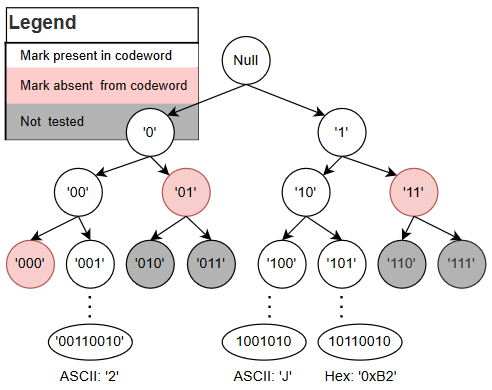
\includegraphics[scale=.59]{images/decoder_search_tree.png}
     \caption{Partial Decoder Tree. }
     \label{treeimag}
 \end{figure}

In this example, at a depth of 3, the search has eliminated 5/8 of the future substrings. In other words, the decoder has already eliminated about 40,962 of the 65,536 message possibilities. While helpful to understand the efficiency of the BBC decoder, this top-down perspective suggests a breadth-first search. Note that because the algorithm is depth-first, the decoder would not discover the ‘1’ branch of the tree until the message ‘00110010’ had been fully decoded. The terminal nodes at the bottom of the tree show that the RX-codec decoded ‘2’, ‘J’, and 0xB2. In this case, with $\mu=0.375$, there were 2 hallucinations.
 
However, in the presence of jamming, the packet density is more consequential than the original codeword density; the channel bitwise-OR will introduce more marks than were in the original packet. For example, when the encoded ‘2’ is jammed by interference that represents a BBC-encoded ‘!,’ 4 new marks are added and packet density is $\frac{6+5}{16}=0.6875$. 

\begin{table}[h]
\label{BBC Packet}
    \centering
    \caption{Channel OR. }
    \begin{center}
    \begin{tabular}{ | m{10em} | m{1.2cm}| m{2.35cm} | } 
      \hline
      Origin & ASCII Character & BBC Codeword \\ 
      \hline
      Original message (TX) & 2 &  10011100  00001010\\ 
      \hline
      Jamming signal        & ! &  01000001  10001101\\ 
      \hline
      Channel packet (OR)   &  N/A &  11011101  10001111 \\ 
      \hline
    \end{tabular}
    \end{center}
\end{table}

Now over the 0.5 threshold, the decoder returns 14 possibilities (8 of which are ASCII characters)—a comparable result to the ASCII-only encoder. This example demonstrates the importance of judiciously sizing the BBC codeword. In the same jamming scenario, the decoder finds 5 message possibilities if a 32-bit codeword is used. With a 56-bit codeword, no hallucinations are present: only ‘2’ and ‘!’ remain. 

\section{The Glowworm Hash}

Baird, Bahn, Carlisle, and Smith designed an optimal mark-placing hash function for BBC called Glowworm \cite{glowworm}. Originally written as C macro functions, the code has been translated to Python to support object-oriented integration in GNURadio. This hash is comprised of 3 functions: one for initializing a shift register, one to process a bit and return a mark index, and one to restore the shift register’s state after processing a bit (i.e., a bit deletion). The \textit{init()} function fills up a shift register with 32 64-bit words. The initial hash state is determined by 4096 iterations of adding the previous entry’s least significant bit. 

\begin{figure}[h]
    \centering
    \begin{lstlisting}[language=Python]
    # Initialize Glowworm
    def init(s):
        n = 0
        h = 1
        for i in range(32):
            s[i]=0
        for i in range(4096):
            h=add_bit(h&1, s)
        n = 0
    \end{lstlisting}
    \caption{Glowworm Initialization Function. }
    \label{gwHashInit}
 \end{figure}

The \textit{add\_bit()} function actually hashes a given bit. In BBC, the modulo of its 64-bit return and the codeword length becomes the index of the new mark. In order to "hash a substring," each individual bit needs to be hashed in order. The shift register's modified state is responsible for ‘01’ giving a different output than ‘1’ or ‘001’; it can essentially store a substring even though it is passed via $n$ separate function calls, where $n$ is the length of the current substring and a global variable.  

\begin{figure}[h]
    \centering
    \begin{lstlisting}[language=Python]
    # Enforce 64-bit word
    MAX_VAL = 0xffffffffffffffff
    
    # Hash a bit
    def add_bit(b, s):
        t = (s[n % 32]^(0xffffffff if b else 0))
        t = ((t|(t>>1))^((t<<1)&MAX_VAL))
        t = (t ^ (t>>4)^(t>>8)^(t>>16)^(t>>32))
        n += 1                           
        s[n % 32] ^= (t&MAX_VAL)
        return s[n % 32] 
    \end{lstlisting}
    \caption{Glowworm Hash Function. }
    \label{gwHashAdd}
 \end{figure}

 Finally, the \textit{del\_bit()} function reverses a hash state change caused by add\_bit(). This enables the BBC decoder to navigate the search tree; in cases where a substring’s mark is not found in the codeword, del\_bit() unhashes the last bit and traverses one level up in the tree.

 \begin{figure}[h]
    \centering
    \begin{lstlisting}[language=Python]
    def del_bit(b, s):
        n -= 1
        add_bit(b,s), 
        n -= 1
        return s[n % 32]
    \end{lstlisting}  
    \caption{Glowworm Reverse Hash Function. }  
    \label{gwHashDel}
 \end{figure}  



\section{Implementation of BBC in Python}
Python’s support of object oriented programming enables the creation of a BBC codec object that can simultaneously encode messages and decode codewords. This is advantageous toward supporting full duplex wireless communication, rather than relying on procedural scripts. Furthermore, Python’s built-in bytearry object supports a variable-length array that can store more information than a machine-precise 64-bit word. This is particularly helpful for creating large codewords (e.g., $2^{20}$ bits long). Since the bytearray object supports indexing via the \textit{memoryview()} method, it is easy to place and search for BBC marks. The Python \textit{Codec} object initializes both an \textit{Encoder} and a \textit{Decoder} for predetermined message, and codeword, and checksum lengths \ref{PyCodec}. Note that BBC performs a pseudo-checksum by appending additional zeros to the message before encoding it, reducing the number of hallucinations contained in the codeword.

To create a BBC codeword, data is parsed from the source, interpolated to \textit{message\_length}-long bit vectors, and passed to the \textit{Encoder}. Once its Glowworm shift register has been initialized (lines 11-14), it is free to iteratively place marks for each substring in the message (lines 27-34). Only one bit is hashed at a time, but the shift register stores the rest of the substring until bits are deleted from it \ref{PyEncoder}.

To decode a BBC codeword, an iterative model is used, rather than the recursive model proposed in \cite{thesis}. This novel approach increases efficiency and reduces the stack size, making it computationally easier to decode larger packets/codewords. Messages that have a mark in the codeword for each substring are stored in the static variable, \textit{message\_list} \ref{PyDecoder}.

To iterate the depth-first search, the decoder uses Glowworm to check if it can append a 0 to the current message substring, which is initially empty. If Glowworm returns an index where a mark is present in the codeword, the current substring is valid, and the "explore" path is taken (lines 33-48). If the current substring is not covered by the packet, then the "backtrace" path is taken (lines 51-72). Here, the algorithm can reliably take the next "deepest" path by deleting 1's from the end of the current message substring until a 0 is encountered (reducing its depth), at which point it changes that 0 to a 1 and continues to the next iteration. After every message covered message is found, they are all returned via \textit{message\_list} (line 75) \ref{PyDecoder}.

\section{Implementation of BBC in GNURadio}
To support SDR testing, the \textit{Encoder} and \textit{Decoder} are each implemented as a GNURadio \textit{Python Blocks}. The class implementations are similar; however, each is instantiated in the respective \textit{blk} constructor \ref{GnuEncodeAppendix}. These custom blocks along with native \textit{Stream to Vector} and \textit{Vector to Stream} blocks serve as a basic testbed for BBC/CCSS in GNURadio, leaving the modulation and jamming strategies open for implementation.  

Initial verification consisted of a simulation, as shown in Figure \ref{fig:bbc_sim}. Due to the ambivalence of the BBC codec to extra marks, it is capable of encoding multiple messages into a single codeword; this flowgraph demonstrates this capability by encoding the two messages separately and performing a bitwise "OR" on the two resulting codewords. The final codeword is then translated and decoded with no errors. In this implementation, the codeword length and message length are known by the encoder and decoder. The BBC encoder and encoder expect vectors of the same length as the message and codeword as inputs/outputs, respectively. Stream-to-vector and vector-to-stream blocks manage the data flow appropriately. In fact, one of the main challenges of developing the encoder and decoder block is to dynamically scale the size of the input and output vectors for the encoder and decoders to match arbitrary message and codeword lengths. At one point, a pull request existed to implement this functionality within the core GNURadio source code, but it was closed without remedy \cite{grcissue}. 

As was previously mentioned, it is crucial to correctly size the codeword to remain under 50\% mark density. Testing of our GNURadio implementation proved this limit. We performed two separate tests to verify this limit. 

First, using a 128-byte ($2^{7}$) message and various codeword lengths from $2^{17}$ to $2^8$ bytes, the original message was recovered until the codeword reached $2^9$ bytes. At this point, the decoder produced a 1-byte error, in which the final character was not correctly decoded. Reducing the codeword length further to $2^8$ bytes resulted in complete failure of the codeword to produce a message. 

Secondly, we used the simulation to investigate the effect of extra marks on the decoded messages. Figure \ref{fig:bbc_fake_news} illustrates the flowgraph. In this case, a single byte is OR'd with the codeword to produce extra marks wtihin each byte of the codeword. As expected, byte values containing three 1's (such as the 00011010$_2$ = 26$_{10}$) did not significantly affect the decoding process, since the mark density was still below the 50\% threshold. However, values such as 00011011$_2$ = 27$_{10}$ produced a failure in the decoder. 

Use of a significant codeword-to-message ratio (such as $2^{10}$) negates any significant errors induced by jamming or noise, as the mark density of the original codeword will be so small as to allow for a significant number of fake marks 

\begin{figure}[h]
    \centering
    \includegraphics[scale=0.25]{./figures/GRCCodec_Multiple Messages_V2}
    \caption{The generic BBC decoder simulation as implemented in GNURadio. }
    \label{fig:bbc_sim}
\end{figure}

\begin{figure}[h]
    \centering
    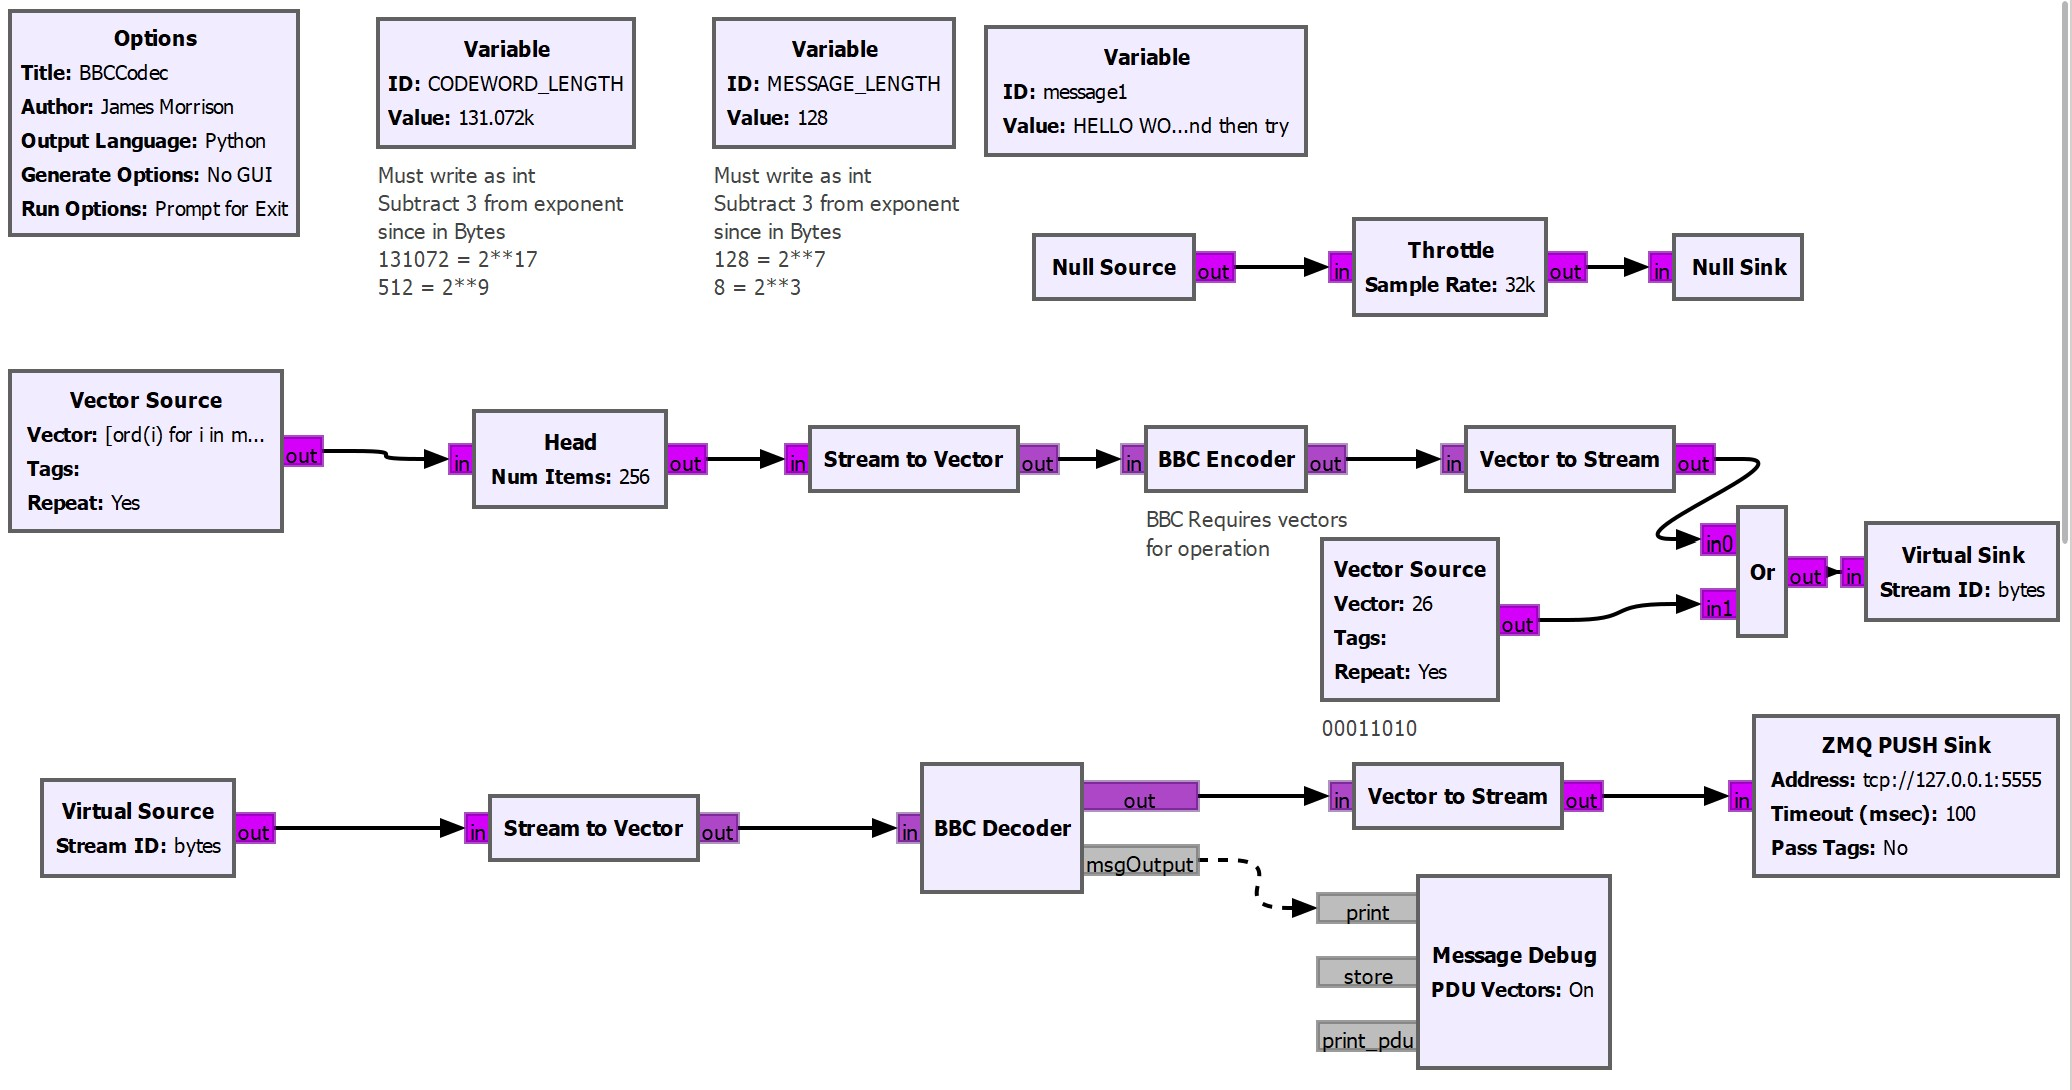
\includegraphics[scale=0.25]{./figures/GRCCodec_Fake marks}
    \caption{The generic BBC decoder simulation modified for injecting fake marks into a codeword.}
    \label{fig:bbc_fake_news}
\end{figure}

\section{Towards Hardware Verification}
The next logical step is to incorporate the BBC encoder/decoder framework into a representative modulation scheme. Bahn \cite{thesis} advises against any constant envelope modulation schemes, as such jamming in schemes do not act as bitwise OR functions. Therefore, we opted for a straightforward OOK modulation scheme, as shown in Figures \ref{fig:bbc_ook_tx} and \ref{fig:bbc_ook_rx}. 

Although most of the blocks are standard GRC blocks, the OOK decoder is a custom python blocks, which serves to decode the received and filtered OOK signal. Since each bit in the codeword is repeated to allow for modulation of a full period of the carrier, the received and demodulated signal must be carefully sampled for correct decoding. In this case, the received samples are counted and a correlated into the appropriate bit value (1 or 0). This particular block takes advantage of the PMT data type to output codewords; this is simply for convenience and will be updated in the near future. The detected bits are sent as individually bytes using the PMT.inter() method. In the future, these bytes will be sent over a standard output port. 

To We modified the BBC decoder from the simulation stage to receive the individual bytes and compile the codeword, which is fed into the glowworm decoding algorithm. 

In order to assess the performance of the BBC OOK implementation, the transmission time was compared with an OOK simulation containing no BBC blocks and the same custom OOK decoder, transmitting a 512 byte message. The difference in performance between the two execution times was negligible. 


\begin{figure}
    \centering
    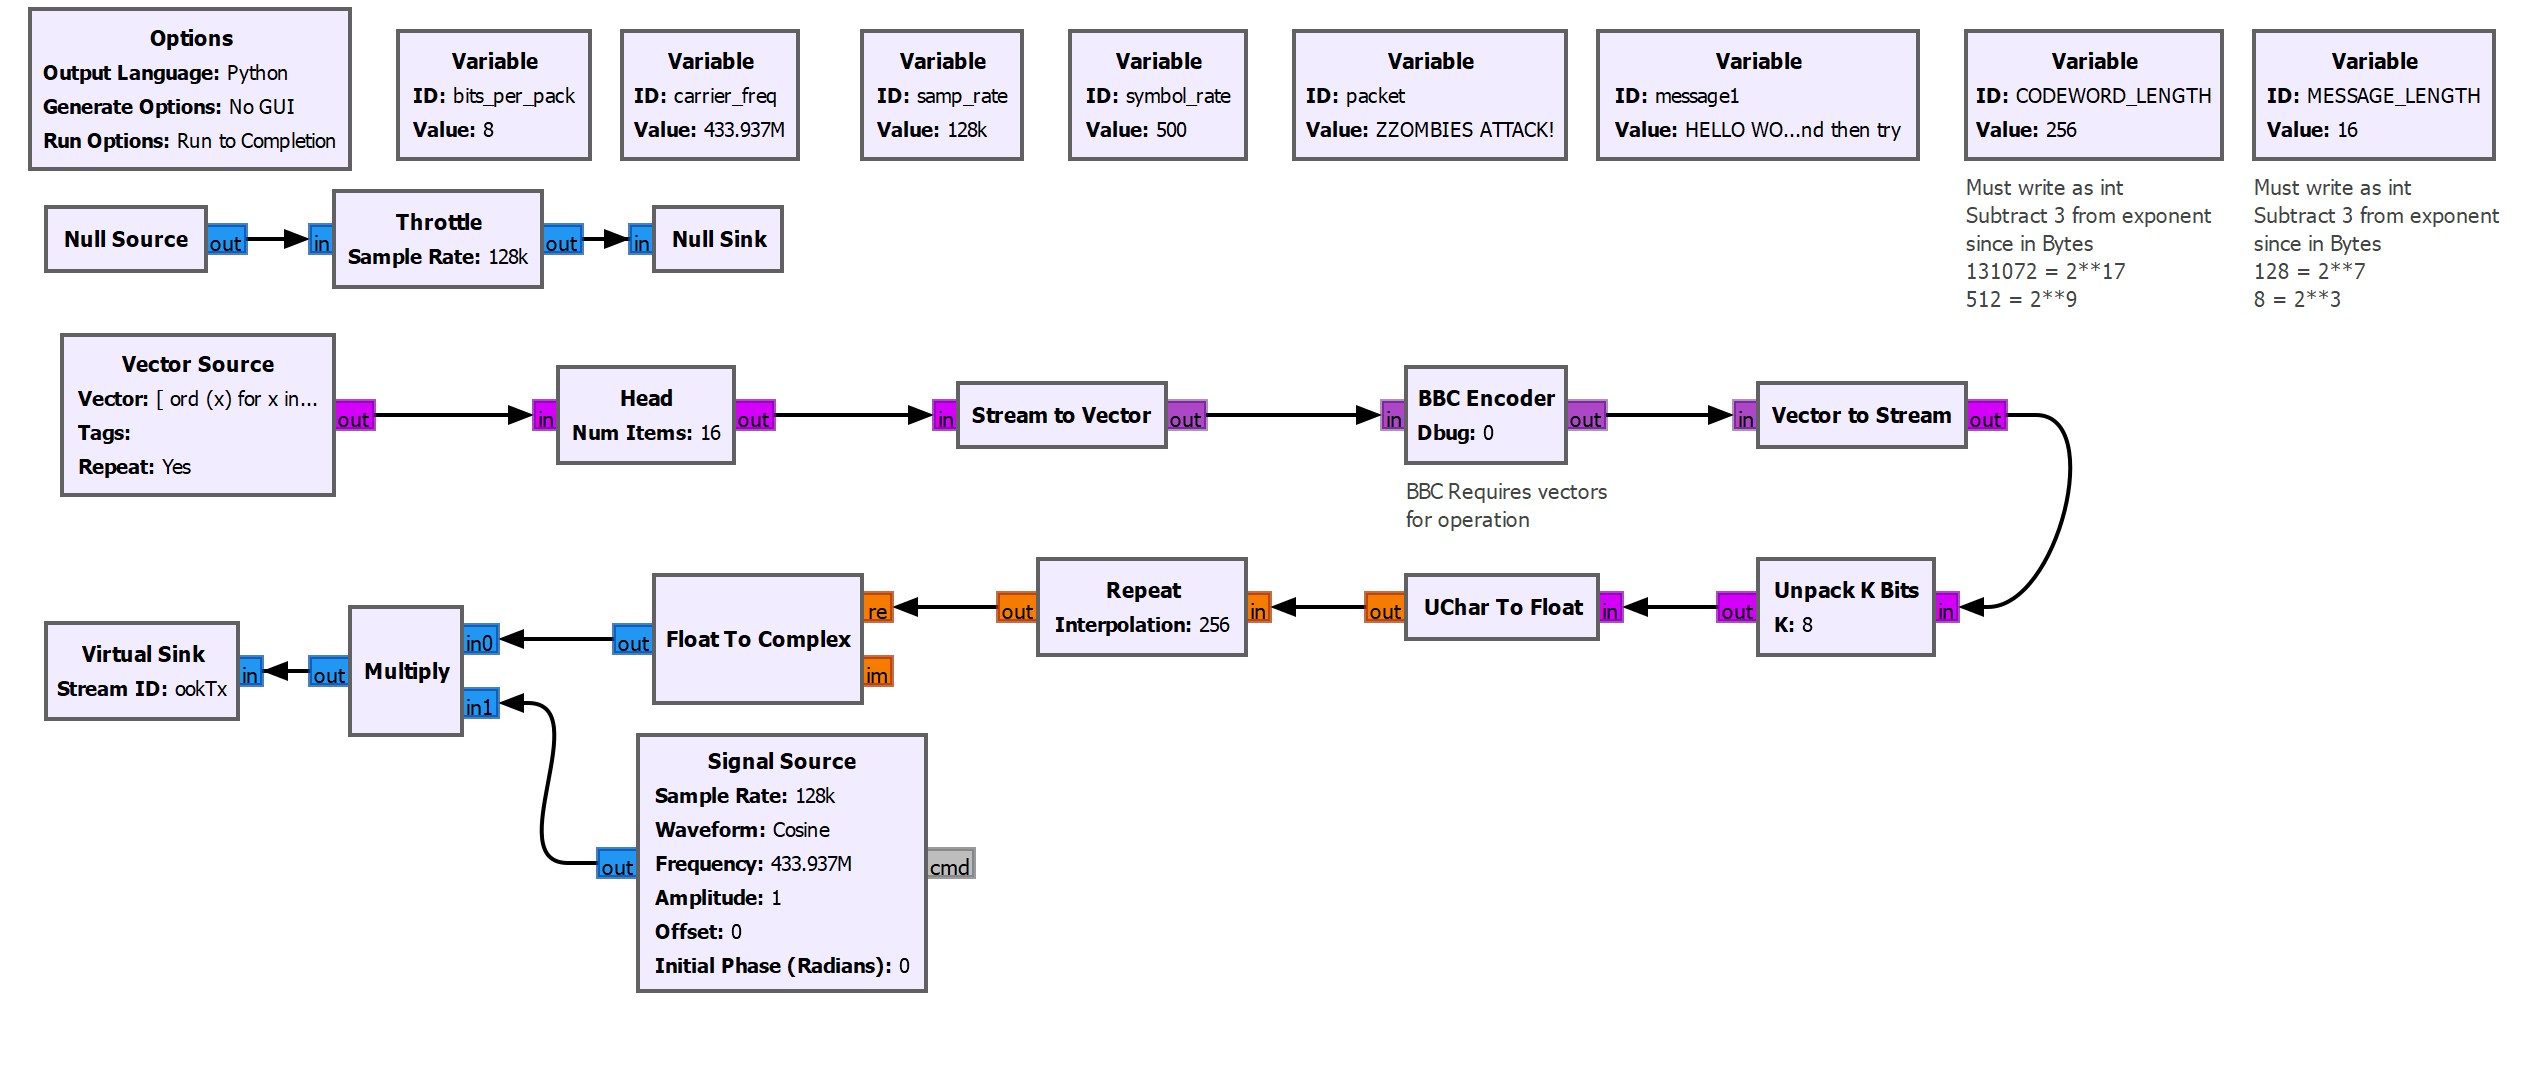
\includegraphics[scale=0.25]{./figures/bbc_ook_1}
    \caption{The BBC encoder coupled with an OOK transmitter.}
    \label{fig:bbc_ook_tx}
\end{figure}


\begin{figure}
    \centering
    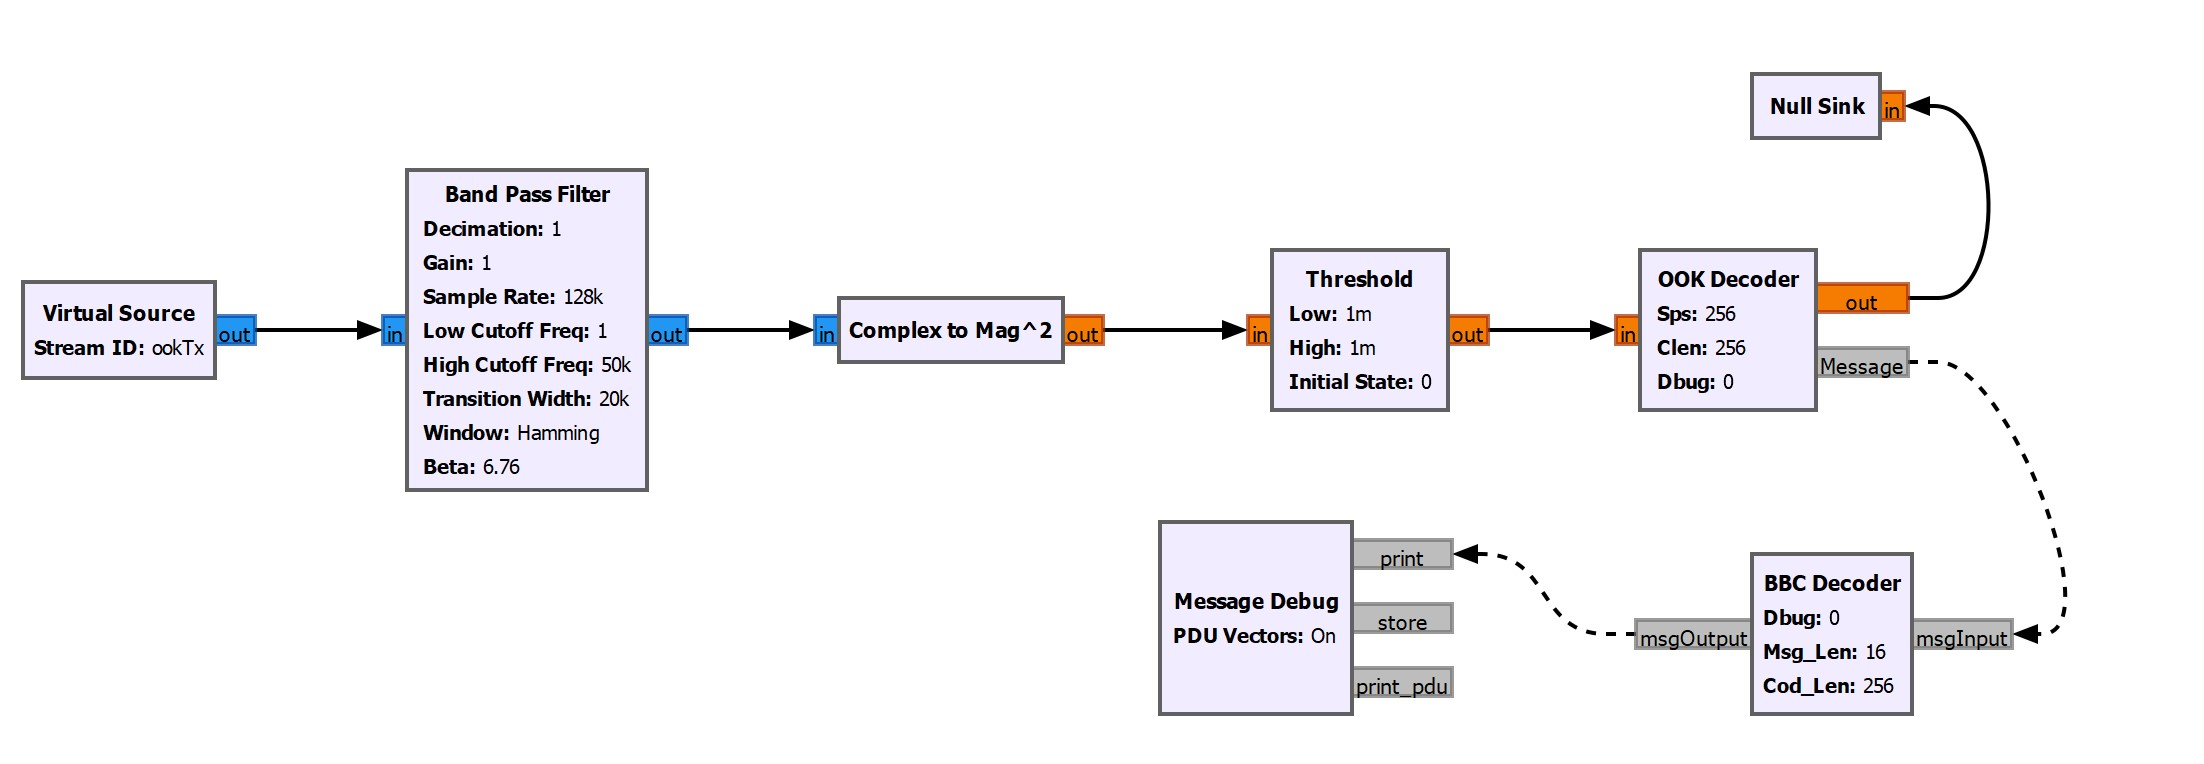
\includegraphics[scale=0.25]{./figures/bbc_ook_2}
    \caption{The BBC decoder coupled with an OOK receiver/decoder.}
    \label{fig:bbc_ook_rx}
\end{figure}

\newpage
\section{Conclusions and Future Work}

Lessons Learned   
-   \newline
-  \newline

     
More work is needed to develop the robustness of and use-cases for BBC real-world integration. First, there are theoretical performance upgrades to the base algorithm. These include multimark BBC, codeword detection, checksum implementation, and active statistic thresholding.   

Secondly, further modeling would help improve performance and efficiency. Predicted performance metrics would help inform message, codeword, and checksum length selection for variable data-rates and expected jamming/noise powers. Specific to the encoder, these metrics include codeword density and overlap count, as functions of codeword and message legnths. For the decoder, they include expected packet density and decode time-complexity, as functions of codeword and message lengths and expected channel noise.   

Finally, rigorous and thorough testing of BBC under diverse noise and jamming strategies must be conducted to prove the algorithm's worth. From a communications perspective, reducing the probability of mark-deletion necessarily increases the probability that an erroneous mark is added-- the extent of this change has not been tested and is dependent on the selected modulation technique.


\bibliographystyle{IEEEtran}
\nocite{*}
\bibliography{refs}

\onecolumn
\newpage

\renewcommand\thesubsection{\arabic{subsection}}

\appendices
\section{BBC Python Code}

%\subsection{BBC Python Code}
%\label{Python}

\subsection{Codec Class}
\label{PyCodec}
\lstset{style=2ndstyle}
\begin{lstlisting}[language=Python]
class Codec:
    # The codec is comprised of an encoder and decoder, with an associated message/codeword pair
    def __init__(self, MSG_LEN, COD_LEN, CHK_LEN):
        self.MSG_LEN = MSG_LEN
        self.COD_LEN = COD_LEN
        self.CHK_LEN = CHK_LEN
        self.encoder = Encoder(self.MSG_LEN, self.COD_LEN, self.CHK_LEN)
        self.decoder = Decoder(self.MSG_LEN, self.COD_LEN, self.CHK_LEN)

    # Resulting functionality should be "mycodec.encode(<message as a string>)"
    def bbc_encode(self, message):
        self.encoder = Encoder(self.MSG_LEN, self.COD_LEN, self.CHK_LEN)
        return self.encoder.encode(message)

    # Resulting functionality should be "mycodec.decode(bytearray1)"
    def bbc_decode(self, codeword):
        self.decoder = Decoder(self.MSG_LEN, self.COD_LEN, self.CHK_LEN)
        return self.decoder.decode(codeword)
\end{lstlisting}  


\subsection{Encoder Class}
\label{PyEncoder}
\begin{lstlisting}[language=Python]
import glowworm.py as gw

class Encoder:
    def __init__(self, MSG_LEN, COD_LEN, CHK_LEN):
        self.shift_register = self.init_shift_register()
        self.MSG_LEN = MSG_LEN
        self.COD_LEN = COD_LEN
        self.CHK_LEN = CHK_LEN

    # Create a shift register using Glowworm
    def init_shift_register(self):
        shift_register = [0 for i in range(32)]
        gw.init(shift_register)
        return (shift_register)

    # Force message to be correct length of bytes in ASCII
    def parse_input(self, input):
        input = input.encode(encoding="ASCII")
        message = bytearray(int(self.MSG_LEN/8))
        memoryview(message)[0:(len(input))] = input
        return message

    # Encode a message using the BBC algorithm
    def encode(self, input):
        message = self.parse_input(input)
        codeword = bytearray(int(self.COD_LEN/8))
        for i in range(self.MSG_LEN):
            # ASCII byte to be encoded
            element = memoryview(message)[int((i-i%8)/8)]
            bit = ((element) >> (i%8)) & 0b1
            # Extract bit from Byte
            mark_loc = gw.add_bit(bit, self.shift_register) % self.COD_LEN
            # Mark location from glowworm
            memoryview(codeword)[int((mark_loc-mark_loc%8)/8)] |= 1<<(mark_loc%8)
        return(codeword)
\end{lstlisting} 
    

\newpage
\subsection{Decoder Class}
\label{PyDecoder}
\begin{lstlisting}[language=Python]
from math import ceil
import glowworm.py as gw

class Decoder:
    # Store configuration parameters as static variables
    def __init__(self, MSG_LEN, COD_LEN, CHK_LEN):
        # <Constructor here>


    # Allocate memory for and initialize the shift register
    def init_shift_register(self):
        shift_register = [0 for i in range(32)]
        gw.init(shift_register)
        return (shift_register)

    # Use novel iterative approach to decoding a packet
    def decode(self, packet):
    
        # Initialize variables
        self.message_list = []
        message = bytearray(ceil((self.MSG_LEN + self.CHK_LEN)/8))

        while True:
            # Find the proposed bit from previous execution, or a 0 if initial iteration
            prop_bit = (memoryview(message)[int((self.n - self.n%8)/8)]>>(self.n%8)) & 0b1
            
            # Find the corresponding mark location from glowworm
            val = gw.add_bit(prop_bit, self.shift_register) % (self.COD_LEN)
            
            # Logical AND to determine if present in packet/codeword
            bit = (memoryview(packet)[int((val-val%8)/8)]>>(val%8)) & 0b1

            # If the mark is present, explore
            if bit==1:
                # Message is complete, write to buffer
                if self.n == (self.MSG_LEN + self.CHK_LEN - 1):
                    self.message_list.append(bytes(memoryview(message)\
                                                   [0:self.MSG_LEN - 1 - self.CHK_LEN]))
                    bit = 0
                    
                # Message is incomplete, continue assuming next bit is 0
                elif self.n < (self.MSG_LEN + self.CHK_LEN - 1):
                    self.n += 1
                    memoryview(message)[int((self.n - self.n%8)/8)] &= (0xff ^ (1<<self.n%8))
                    continue
                    
            # If the mark is not present, backtrace
            if bit!=1:
                # Delete checksum bits
                while self.n >= self.MSG_LEN: 
                    gw.del_bit(0, self.shift_register)
                    self.n -= 1
                    
                # Delete 1's until a 0 is encountered
                while self.n >=0 and (((memoryview(message)[int((self.n - self.n%8)/8)]>>\
                                                                (self.n%8)) & 0b1 )==1):
                    gw.del_bit(1, self.shift_register)
                    memoryview(message)[int((self.n - self.n%8)/8)] &= (0xff ^ (1<<self.n%8))
                    self.n -= 1
                    
                # Packet is fully decoded, proceed with next packet
                if self.n < 0: 
                    break
                    
                # Move over to the 1 branch of current search
                else: 
                    gw.del_bit(0, self.shift_register)
                    memoryview(message)[int((self.n - self.n%8)/8)] |= (1<<self.n%8)

        return self.message_list
\end{lstlisting} 

\newpage
\section{GNURadio Implementation}
\subsection{Top-Level Chart}
\label{GnuTopLevel}
    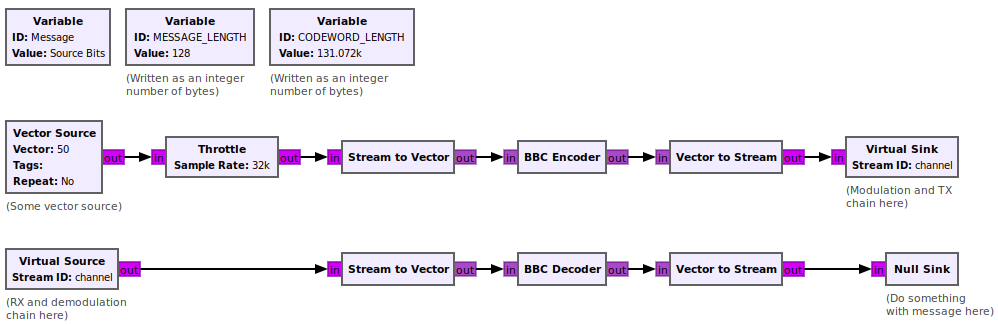
\includegraphics[scale=.6]{images/BBC grc.png}

\subsection{GNURadio Encoder Block Class}
\label{GnuEncodeAppendix}
\begin{lstlisting}[language=Python]
from gnuradio import gr
import numpy as np

class blk(gr.sync_block):

    # Configure port sizes
    def __init__(self, MESSAGE_LENGTH=2**7, CODEWORD_LENGTH=2**17):
        self.msg_len = MESSAGE_LENGTH
        self.cod_len = CODEWORD_LENGTH

        # Use a synchronous block
        gr.sync_block.__init__(self,
            name='BBC Encoder',
            in_sig =[(np.byte, self.msg_len)],    
            out_sig=[(np.byte, self.cod_len)])
        
        # Convert from Bytes to bits
        self.myEncoder = Encoder(self.msg_len*8, self.cod_len*8)
    
    # Use BBC to encode the incoming message vectors
    def work(self, input_items, output_items):
        result = self.myEncoder.encode(input_items[0][:])        
        try:
            output_items[0][:] = result
            return len(output_items[0])
        except:
            raise RuntimeError("BBC Encoder output assignment failed")
\end{lstlisting}

\newpage
\subsection{GNURadio Decoder Block Class}
\label{GnuDecodeAppendix}
\begin{lstlisting}[language=Python]
from gnuradio import gr
import numpy as np


class blk(gr.interp_block):

    # Configure port sizes
    def __init__(self, MESSAGE_LENGTH=2**7, CODEWORD_LENGTH=2**17):
        self.msg_len = MESSAGE_LENGTH
        self.cod_len = CODEWORD_LENGTH

        # Use an interpolation block
        gr.sync_block.__init__(self,
            name='BBC Decoder',
            in_sig =[(np.byte, self.cod_len)],    
            out_sig=[(np.byte, self.msg_len)])
            
        # Initialize the interpolation rate to synchronous case
        self.set_relative_rate(1)
        
        # Convert from Bytes to bits
        self.myDecoder = Decoder(self.msg_len*8, self.cod_len*8, DEFAULT_CHECKSUM)


    # Use BBC to decode the incoming codeword vectors
    def work(self, input_items, output_items):
        
        # Pull packet from the queue
        packet = input_items[0][:][0]
        
        # Check for a nonzero codeword
        if sum(packet >0):
            
            result = self.myDecoder.decode(packet)
            interp = len(result)
            
            #Check for a decoded message
            if interp > 0:
                
                # Definre the number of outputs
                self.set_relative_rate(interp)
                
                # Assign outputs iteratively
                for j in range(interp):
                    try:
                        output_items[0][j][:] = result[j]
                    except:
                            raise RuntimeError("BBC Encoder output assignment failed")
        return len(output_items)
\end{lstlisting} 

\end{document}
